\documentclass[11pt]{article}

\usepackage[style=numeric-comp,useprefix,hyperref,backend=bibtex]{biblatex}

    \usepackage[breakable]{tcolorbox}
    \usepackage{parskip} % Stop auto-indenting (to mimic markdown behaviour)
    

    % Basic figure setup, for now with no caption control since it's done
    % automatically by Pandoc (which extracts ![](path) syntax from Markdown).
    \usepackage{graphicx}
    % Maintain compatibility with old templates. Remove in nbconvert 6.0
    \let\Oldincludegraphics\includegraphics
    % Ensure that by default, figures have no caption (until we provide a
    % proper Figure object with a Caption API and a way to capture that
    % in the conversion process - todo).
    \usepackage{caption}
    \DeclareCaptionFormat{nocaption}{}
    \captionsetup{format=nocaption,aboveskip=0pt,belowskip=0pt}
    \usepackage{animate}

    \usepackage{float}
    \floatplacement{figure}{H} % forces figures to be placed at the correct location
    \usepackage{xcolor} % Allow colors to be defined
    \usepackage{enumerate} % Needed for markdown enumerations to work
    \usepackage{geometry} % Used to adjust the document margins
    \usepackage{amsmath} % Equations
    \usepackage{amssymb} % Equations
    \usepackage{textcomp} % defines textquotesingle
    % Hack from http://tex.stackexchange.com/a/47451/13684:
    \AtBeginDocument{%
        \def\PYZsq{\textquotesingle}% Upright quotes in Pygmentized code
    }
    \usepackage{upquote} % Upright quotes for verbatim code
    \usepackage{eurosym} % defines \euro

    \usepackage{iftex}
    \ifPDFTeX
        \usepackage[T1]{fontenc}
        \IfFileExists{alphabeta.sty}{
              \usepackage{alphabeta}
          }{
              \usepackage[mathletters]{ucs}
              \usepackage[utf8x]{inputenc}
          }
    \else
        \usepackage{fontspec}
        \usepackage{unicode-math}
    \fi

    \usepackage{fancyvrb} % verbatim replacement that allows latex
    \usepackage{grffile} % extends the file name processing of package graphics
                         % to support a larger range
    \makeatletter % fix for old versions of grffile with XeLaTeX
    \@ifpackagelater{grffile}{2019/11/01}
    {
      % Do nothing on new versions
    }
    {
      \def\Gread@@xetex#1{%
        \IfFileExists{"\Gin@base".bb}%
        {\Gread@eps{\Gin@base.bb}}%
        {\Gread@@xetex@aux#1}%
      }
    }
    \makeatother
    \usepackage[Export]{adjustbox} % Used to constrain images to a maximum size
    \adjustboxset{max size={0.9\linewidth}{0.9\paperheight}}

    % The hyperref package gives us a pdf with properly built
    % internal navigation ('pdf bookmarks' for the table of contents,
    % internal cross-reference links, web links for URLs, etc.)
    \usepackage{hyperref}
    % The default LaTeX title has an obnoxious amount of whitespace. By default,
    % titling removes some of it. It also provides customization options.
    \usepackage{titling}
    \usepackage{longtable} % longtable support required by pandoc >1.10
    \usepackage{booktabs}  % table support for pandoc > 1.12.2
    \usepackage{array}     % table support for pandoc >= 2.11.3
    \usepackage{calc}      % table minipage width calculation for pandoc >= 2.11.1
    \usepackage[inline]{enumitem} % IRkernel/repr support (it uses the enumerate* environment)
    \usepackage[normalem]{ulem} % ulem is needed to support strikethroughs (\sout)
                                % normalem makes italics be italics, not underlines
    \usepackage{soul}      % strikethrough (\st) support for pandoc >= 3.0.0
    \usepackage{mathrsfs}
    

    
    % Colors for the hyperref package
    \definecolor{urlcolor}{rgb}{0,.145,.698}
    \definecolor{linkcolor}{rgb}{.71,0.21,0.01}
    \definecolor{citecolor}{rgb}{.12,.54,.11}

    % ANSI colors
    \definecolor{ansi-black}{HTML}{3E424D}
    \definecolor{ansi-black-intense}{HTML}{282C36}
    \definecolor{ansi-red}{HTML}{E75C58}
    \definecolor{ansi-red-intense}{HTML}{B22B31}
    \definecolor{ansi-green}{HTML}{00A250}
    \definecolor{ansi-green-intense}{HTML}{007427}
    \definecolor{ansi-yellow}{HTML}{DDB62B}
    \definecolor{ansi-yellow-intense}{HTML}{B27D12}
    \definecolor{ansi-blue}{HTML}{208FFB}
    \definecolor{ansi-blue-intense}{HTML}{0065CA}
    \definecolor{ansi-magenta}{HTML}{D160C4}
    \definecolor{ansi-magenta-intense}{HTML}{A03196}
    \definecolor{ansi-cyan}{HTML}{60C6C8}
    \definecolor{ansi-cyan-intense}{HTML}{258F8F}
    \definecolor{ansi-white}{HTML}{C5C1B4}
    \definecolor{ansi-white-intense}{HTML}{A1A6B2}
    \definecolor{ansi-default-inverse-fg}{HTML}{FFFFFF}
    \definecolor{ansi-default-inverse-bg}{HTML}{000000}

    % common color for the border for error outputs.
    \definecolor{outerrorbackground}{HTML}{FFDFDF}

    % commands and environments needed by pandoc snippets
    % extracted from the output of `pandoc -s`
    \providecommand{\tightlist}{%
      \setlength{\itemsep}{0pt}\setlength{\parskip}{0pt}}
    \DefineVerbatimEnvironment{Highlighting}{Verbatim}{commandchars=\\\{\}}
    % Add ',fontsize=\small' for more characters per line
    \newenvironment{Shaded}{}{}
    \newcommand{\KeywordTok}[1]{\textcolor[rgb]{0.00,0.44,0.13}{\textbf{{#1}}}}
    \newcommand{\DataTypeTok}[1]{\textcolor[rgb]{0.56,0.13,0.00}{{#1}}}
    \newcommand{\DecValTok}[1]{\textcolor[rgb]{0.25,0.63,0.44}{{#1}}}
    \newcommand{\BaseNTok}[1]{\textcolor[rgb]{0.25,0.63,0.44}{{#1}}}
    \newcommand{\FloatTok}[1]{\textcolor[rgb]{0.25,0.63,0.44}{{#1}}}
    \newcommand{\CharTok}[1]{\textcolor[rgb]{0.25,0.44,0.63}{{#1}}}
    \newcommand{\StringTok}[1]{\textcolor[rgb]{0.25,0.44,0.63}{{#1}}}
    \newcommand{\CommentTok}[1]{\textcolor[rgb]{0.38,0.63,0.69}{\textit{{#1}}}}
    \newcommand{\OtherTok}[1]{\textcolor[rgb]{0.00,0.44,0.13}{{#1}}}
    \newcommand{\AlertTok}[1]{\textcolor[rgb]{1.00,0.00,0.00}{\textbf{{#1}}}}
    \newcommand{\FunctionTok}[1]{\textcolor[rgb]{0.02,0.16,0.49}{{#1}}}
    \newcommand{\RegionMarkerTok}[1]{{#1}}
    \newcommand{\ErrorTok}[1]{\textcolor[rgb]{1.00,0.00,0.00}{\textbf{{#1}}}}
    \newcommand{\NormalTok}[1]{{#1}}

    % Additional commands for more recent versions of Pandoc
    \newcommand{\ConstantTok}[1]{\textcolor[rgb]{0.53,0.00,0.00}{{#1}}}
    \newcommand{\SpecialCharTok}[1]{\textcolor[rgb]{0.25,0.44,0.63}{{#1}}}
    \newcommand{\VerbatimStringTok}[1]{\textcolor[rgb]{0.25,0.44,0.63}{{#1}}}
    \newcommand{\SpecialStringTok}[1]{\textcolor[rgb]{0.73,0.40,0.53}{{#1}}}
    \newcommand{\ImportTok}[1]{{#1}}
    \newcommand{\DocumentationTok}[1]{\textcolor[rgb]{0.73,0.13,0.13}{\textit{{#1}}}}
    \newcommand{\AnnotationTok}[1]{\textcolor[rgb]{0.38,0.63,0.69}{\textbf{\textit{{#1}}}}}
    \newcommand{\CommentVarTok}[1]{\textcolor[rgb]{0.38,0.63,0.69}{\textbf{\textit{{#1}}}}}
    \newcommand{\VariableTok}[1]{\textcolor[rgb]{0.10,0.09,0.49}{{#1}}}
    \newcommand{\ControlFlowTok}[1]{\textcolor[rgb]{0.00,0.44,0.13}{\textbf{{#1}}}}
    \newcommand{\OperatorTok}[1]{\textcolor[rgb]{0.40,0.40,0.40}{{#1}}}
    \newcommand{\BuiltInTok}[1]{{#1}}
    \newcommand{\ExtensionTok}[1]{{#1}}
    \newcommand{\PreprocessorTok}[1]{\textcolor[rgb]{0.74,0.48,0.00}{{#1}}}
    \newcommand{\AttributeTok}[1]{\textcolor[rgb]{0.49,0.56,0.16}{{#1}}}
    \newcommand{\InformationTok}[1]{\textcolor[rgb]{0.38,0.63,0.69}{\textbf{\textit{{#1}}}}}
    \newcommand{\WarningTok}[1]{\textcolor[rgb]{0.38,0.63,0.69}{\textbf{\textit{{#1}}}}}


    % Define a nice break command that doesn't care if a line doesn't already
    % exist.
    \def\br{\hspace*{\fill} \\* }
    % Math Jax compatibility definitions
    \def\gt{>}
    \def\lt{<}
    \let\Oldtex\TeX
    \let\Oldlatex\LaTeX
    \renewcommand{\TeX}{\textrm{\Oldtex}}
    \renewcommand{\LaTeX}{\textrm{\Oldlatex}}
    % Document parameters
    % Document title
    \title{lezione1}
    
    
    
    
    
    
    
% Pygments definitions
\makeatletter
\def\PY@reset{\let\PY@it=\relax \let\PY@bf=\relax%
    \let\PY@ul=\relax \let\PY@tc=\relax%
    \let\PY@bc=\relax \let\PY@ff=\relax}
\def\PY@tok#1{\csname PY@tok@#1\endcsname}
\def\PY@toks#1+{\ifx\relax#1\empty\else%
    \PY@tok{#1}\expandafter\PY@toks\fi}
\def\PY@do#1{\PY@bc{\PY@tc{\PY@ul{%
    \PY@it{\PY@bf{\PY@ff{#1}}}}}}}
\def\PY#1#2{\PY@reset\PY@toks#1+\relax+\PY@do{#2}}

\@namedef{PY@tok@w}{\def\PY@tc##1{\textcolor[rgb]{0.73,0.73,0.73}{##1}}}
\@namedef{PY@tok@c}{\let\PY@it=\textit\def\PY@tc##1{\textcolor[rgb]{0.24,0.48,0.48}{##1}}}
\@namedef{PY@tok@cp}{\def\PY@tc##1{\textcolor[rgb]{0.61,0.40,0.00}{##1}}}
\@namedef{PY@tok@k}{\let\PY@bf=\textbf\def\PY@tc##1{\textcolor[rgb]{0.00,0.50,0.00}{##1}}}
\@namedef{PY@tok@kp}{\def\PY@tc##1{\textcolor[rgb]{0.00,0.50,0.00}{##1}}}
\@namedef{PY@tok@kt}{\def\PY@tc##1{\textcolor[rgb]{0.69,0.00,0.25}{##1}}}
\@namedef{PY@tok@o}{\def\PY@tc##1{\textcolor[rgb]{0.40,0.40,0.40}{##1}}}
\@namedef{PY@tok@ow}{\let\PY@bf=\textbf\def\PY@tc##1{\textcolor[rgb]{0.67,0.13,1.00}{##1}}}
\@namedef{PY@tok@nb}{\def\PY@tc##1{\textcolor[rgb]{0.00,0.50,0.00}{##1}}}
\@namedef{PY@tok@nf}{\def\PY@tc##1{\textcolor[rgb]{0.00,0.00,1.00}{##1}}}
\@namedef{PY@tok@nc}{\let\PY@bf=\textbf\def\PY@tc##1{\textcolor[rgb]{0.00,0.00,1.00}{##1}}}
\@namedef{PY@tok@nn}{\let\PY@bf=\textbf\def\PY@tc##1{\textcolor[rgb]{0.00,0.00,1.00}{##1}}}
\@namedef{PY@tok@ne}{\let\PY@bf=\textbf\def\PY@tc##1{\textcolor[rgb]{0.80,0.25,0.22}{##1}}}
\@namedef{PY@tok@nv}{\def\PY@tc##1{\textcolor[rgb]{0.10,0.09,0.49}{##1}}}
\@namedef{PY@tok@no}{\def\PY@tc##1{\textcolor[rgb]{0.53,0.00,0.00}{##1}}}
\@namedef{PY@tok@nl}{\def\PY@tc##1{\textcolor[rgb]{0.46,0.46,0.00}{##1}}}
\@namedef{PY@tok@ni}{\let\PY@bf=\textbf\def\PY@tc##1{\textcolor[rgb]{0.44,0.44,0.44}{##1}}}
\@namedef{PY@tok@na}{\def\PY@tc##1{\textcolor[rgb]{0.41,0.47,0.13}{##1}}}
\@namedef{PY@tok@nt}{\let\PY@bf=\textbf\def\PY@tc##1{\textcolor[rgb]{0.00,0.50,0.00}{##1}}}
\@namedef{PY@tok@nd}{\def\PY@tc##1{\textcolor[rgb]{0.67,0.13,1.00}{##1}}}
\@namedef{PY@tok@s}{\def\PY@tc##1{\textcolor[rgb]{0.73,0.13,0.13}{##1}}}
\@namedef{PY@tok@sd}{\let\PY@it=\textit\def\PY@tc##1{\textcolor[rgb]{0.73,0.13,0.13}{##1}}}
\@namedef{PY@tok@si}{\let\PY@bf=\textbf\def\PY@tc##1{\textcolor[rgb]{0.64,0.35,0.47}{##1}}}
\@namedef{PY@tok@se}{\let\PY@bf=\textbf\def\PY@tc##1{\textcolor[rgb]{0.67,0.36,0.12}{##1}}}
\@namedef{PY@tok@sr}{\def\PY@tc##1{\textcolor[rgb]{0.64,0.35,0.47}{##1}}}
\@namedef{PY@tok@ss}{\def\PY@tc##1{\textcolor[rgb]{0.10,0.09,0.49}{##1}}}
\@namedef{PY@tok@sx}{\def\PY@tc##1{\textcolor[rgb]{0.00,0.50,0.00}{##1}}}
\@namedef{PY@tok@m}{\def\PY@tc##1{\textcolor[rgb]{0.40,0.40,0.40}{##1}}}
\@namedef{PY@tok@gh}{\let\PY@bf=\textbf\def\PY@tc##1{\textcolor[rgb]{0.00,0.00,0.50}{##1}}}
\@namedef{PY@tok@gu}{\let\PY@bf=\textbf\def\PY@tc##1{\textcolor[rgb]{0.50,0.00,0.50}{##1}}}
\@namedef{PY@tok@gd}{\def\PY@tc##1{\textcolor[rgb]{0.63,0.00,0.00}{##1}}}
\@namedef{PY@tok@gi}{\def\PY@tc##1{\textcolor[rgb]{0.00,0.52,0.00}{##1}}}
\@namedef{PY@tok@gr}{\def\PY@tc##1{\textcolor[rgb]{0.89,0.00,0.00}{##1}}}
\@namedef{PY@tok@ge}{\let\PY@it=\textit}
\@namedef{PY@tok@gs}{\let\PY@bf=\textbf}
\@namedef{PY@tok@ges}{\let\PY@bf=\textbf\let\PY@it=\textit}
\@namedef{PY@tok@gp}{\let\PY@bf=\textbf\def\PY@tc##1{\textcolor[rgb]{0.00,0.00,0.50}{##1}}}
\@namedef{PY@tok@go}{\def\PY@tc##1{\textcolor[rgb]{0.44,0.44,0.44}{##1}}}
\@namedef{PY@tok@gt}{\def\PY@tc##1{\textcolor[rgb]{0.00,0.27,0.87}{##1}}}
\@namedef{PY@tok@err}{\def\PY@bc##1{{\setlength{\fboxsep}{\string -\fboxrule}\fcolorbox[rgb]{1.00,0.00,0.00}{1,1,1}{\strut ##1}}}}
\@namedef{PY@tok@kc}{\let\PY@bf=\textbf\def\PY@tc##1{\textcolor[rgb]{0.00,0.50,0.00}{##1}}}
\@namedef{PY@tok@kd}{\let\PY@bf=\textbf\def\PY@tc##1{\textcolor[rgb]{0.00,0.50,0.00}{##1}}}
\@namedef{PY@tok@kn}{\let\PY@bf=\textbf\def\PY@tc##1{\textcolor[rgb]{0.00,0.50,0.00}{##1}}}
\@namedef{PY@tok@kr}{\let\PY@bf=\textbf\def\PY@tc##1{\textcolor[rgb]{0.00,0.50,0.00}{##1}}}
\@namedef{PY@tok@bp}{\def\PY@tc##1{\textcolor[rgb]{0.00,0.50,0.00}{##1}}}
\@namedef{PY@tok@fm}{\def\PY@tc##1{\textcolor[rgb]{0.00,0.00,1.00}{##1}}}
\@namedef{PY@tok@vc}{\def\PY@tc##1{\textcolor[rgb]{0.10,0.09,0.49}{##1}}}
\@namedef{PY@tok@vg}{\def\PY@tc##1{\textcolor[rgb]{0.10,0.09,0.49}{##1}}}
\@namedef{PY@tok@vi}{\def\PY@tc##1{\textcolor[rgb]{0.10,0.09,0.49}{##1}}}
\@namedef{PY@tok@vm}{\def\PY@tc##1{\textcolor[rgb]{0.10,0.09,0.49}{##1}}}
\@namedef{PY@tok@sa}{\def\PY@tc##1{\textcolor[rgb]{0.73,0.13,0.13}{##1}}}
\@namedef{PY@tok@sb}{\def\PY@tc##1{\textcolor[rgb]{0.73,0.13,0.13}{##1}}}
\@namedef{PY@tok@sc}{\def\PY@tc##1{\textcolor[rgb]{0.73,0.13,0.13}{##1}}}
\@namedef{PY@tok@dl}{\def\PY@tc##1{\textcolor[rgb]{0.73,0.13,0.13}{##1}}}
\@namedef{PY@tok@s2}{\def\PY@tc##1{\textcolor[rgb]{0.73,0.13,0.13}{##1}}}
\@namedef{PY@tok@sh}{\def\PY@tc##1{\textcolor[rgb]{0.73,0.13,0.13}{##1}}}
\@namedef{PY@tok@s1}{\def\PY@tc##1{\textcolor[rgb]{0.73,0.13,0.13}{##1}}}
\@namedef{PY@tok@mb}{\def\PY@tc##1{\textcolor[rgb]{0.40,0.40,0.40}{##1}}}
\@namedef{PY@tok@mf}{\def\PY@tc##1{\textcolor[rgb]{0.40,0.40,0.40}{##1}}}
\@namedef{PY@tok@mh}{\def\PY@tc##1{\textcolor[rgb]{0.40,0.40,0.40}{##1}}}
\@namedef{PY@tok@mi}{\def\PY@tc##1{\textcolor[rgb]{0.40,0.40,0.40}{##1}}}
\@namedef{PY@tok@il}{\def\PY@tc##1{\textcolor[rgb]{0.40,0.40,0.40}{##1}}}
\@namedef{PY@tok@mo}{\def\PY@tc##1{\textcolor[rgb]{0.40,0.40,0.40}{##1}}}
\@namedef{PY@tok@ch}{\let\PY@it=\textit\def\PY@tc##1{\textcolor[rgb]{0.24,0.48,0.48}{##1}}}
\@namedef{PY@tok@cm}{\let\PY@it=\textit\def\PY@tc##1{\textcolor[rgb]{0.24,0.48,0.48}{##1}}}
\@namedef{PY@tok@cpf}{\let\PY@it=\textit\def\PY@tc##1{\textcolor[rgb]{0.24,0.48,0.48}{##1}}}
\@namedef{PY@tok@c1}{\let\PY@it=\textit\def\PY@tc##1{\textcolor[rgb]{0.24,0.48,0.48}{##1}}}
\@namedef{PY@tok@cs}{\let\PY@it=\textit\def\PY@tc##1{\textcolor[rgb]{0.24,0.48,0.48}{##1}}}

\def\PYZbs{\char`\\}
\def\PYZus{\char`\_}
\def\PYZob{\char`\{}
\def\PYZcb{\char`\}}
\def\PYZca{\char`\^}
\def\PYZam{\char`\&}
\def\PYZlt{\char`\<}
\def\PYZgt{\char`\>}
\def\PYZsh{\char`\#}
\def\PYZpc{\char`\%}
\def\PYZdl{\char`\$}
\def\PYZhy{\char`\-}
\def\PYZsq{\char`\'}
\def\PYZdq{\char`\"}
\def\PYZti{\char`\~}
% for compatibility with earlier versions
\def\PYZat{@}
\def\PYZlb{[}
\def\PYZrb{]}
\makeatother


    % For linebreaks inside Verbatim environment from package fancyvrb.
    \makeatletter
        \newbox\Wrappedcontinuationbox
        \newbox\Wrappedvisiblespacebox
        \newcommand*\Wrappedvisiblespace {\textcolor{red}{\textvisiblespace}}
        \newcommand*\Wrappedcontinuationsymbol {\textcolor{red}{\llap{\tiny$\m@th\hookrightarrow$}}}
        \newcommand*\Wrappedcontinuationindent {3ex }
        \newcommand*\Wrappedafterbreak {\kern\Wrappedcontinuationindent\copy\Wrappedcontinuationbox}
        % Take advantage of the already applied Pygments mark-up to insert
        % potential linebreaks for TeX processing.
        %        {, <, #, %, $, ' and ": go to next line.
        %        _, }, ^, &, >, - and ~: stay at end of broken line.
        % Use of \textquotesingle for straight quote.
        \newcommand*\Wrappedbreaksatspecials {%
            \def\PYGZus{\discretionary{\char`\_}{\Wrappedafterbreak}{\char`\_}}%
            \def\PYGZob{\discretionary{}{\Wrappedafterbreak\char`\{}{\char`\{}}%
            \def\PYGZcb{\discretionary{\char`\}}{\Wrappedafterbreak}{\char`\}}}%
            \def\PYGZca{\discretionary{\char`\^}{\Wrappedafterbreak}{\char`\^}}%
            \def\PYGZam{\discretionary{\char`\&}{\Wrappedafterbreak}{\char`\&}}%
            \def\PYGZlt{\discretionary{}{\Wrappedafterbreak\char`\<}{\char`\<}}%
            \def\PYGZgt{\discretionary{\char`\>}{\Wrappedafterbreak}{\char`\>}}%
            \def\PYGZsh{\discretionary{}{\Wrappedafterbreak\char`\#}{\char`\#}}%
            \def\PYGZpc{\discretionary{}{\Wrappedafterbreak\char`\%}{\char`\%}}%
            \def\PYGZdl{\discretionary{}{\Wrappedafterbreak\char`\$}{\char`\$}}%
            \def\PYGZhy{\discretionary{\char`\-}{\Wrappedafterbreak}{\char`\-}}%
            \def\PYGZsq{\discretionary{}{\Wrappedafterbreak\textquotesingle}{\textquotesingle}}%
            \def\PYGZdq{\discretionary{}{\Wrappedafterbreak\char`\"}{\char`\"}}%
            \def\PYGZti{\discretionary{\char`\~}{\Wrappedafterbreak}{\char`\~}}%
        }
        % Some characters . , ; ? ! / are not pygmentized.
        % This macro makes them "active" and they will insert potential linebreaks
        \newcommand*\Wrappedbreaksatpunct {%
            \lccode`\~`\.\lowercase{\def~}{\discretionary{\hbox{\char`\.}}{\Wrappedafterbreak}{\hbox{\char`\.}}}%
            \lccode`\~`\,\lowercase{\def~}{\discretionary{\hbox{\char`\,}}{\Wrappedafterbreak}{\hbox{\char`\,}}}%
            \lccode`\~`\;\lowercase{\def~}{\discretionary{\hbox{\char`\;}}{\Wrappedafterbreak}{\hbox{\char`\;}}}%
            \lccode`\~`\:\lowercase{\def~}{\discretionary{\hbox{\char`\:}}{\Wrappedafterbreak}{\hbox{\char`\:}}}%
            \lccode`\~`\?\lowercase{\def~}{\discretionary{\hbox{\char`\?}}{\Wrappedafterbreak}{\hbox{\char`\?}}}%
            \lccode`\~`\!\lowercase{\def~}{\discretionary{\hbox{\char`\!}}{\Wrappedafterbreak}{\hbox{\char`\!}}}%
            \lccode`\~`\/\lowercase{\def~}{\discretionary{\hbox{\char`\/}}{\Wrappedafterbreak}{\hbox{\char`\/}}}%
            \catcode`\.\active
            \catcode`\,\active
            \catcode`\;\active
            \catcode`\:\active
            \catcode`\?\active
            \catcode`\!\active
            \catcode`\/\active
            \lccode`\~`\~
        }
    \makeatother

    \let\OriginalVerbatim=\Verbatim
    \makeatletter
    \renewcommand{\Verbatim}[1][1]{%
        %\parskip\z@skip
        \sbox\Wrappedcontinuationbox {\Wrappedcontinuationsymbol}%
        \sbox\Wrappedvisiblespacebox {\FV@SetupFont\Wrappedvisiblespace}%
        \def\FancyVerbFormatLine ##1{\hsize\linewidth
            \vtop{\raggedright\hyphenpenalty\z@\exhyphenpenalty\z@
                \doublehyphendemerits\z@\finalhyphendemerits\z@
                \strut ##1\strut}%
        }%
        % If the linebreak is at a space, the latter will be displayed as visible
        % space at end of first line, and a continuation symbol starts next line.
        % Stretch/shrink are however usually zero for typewriter font.
        \def\FV@Space {%
            \nobreak\hskip\z@ plus\fontdimen3\font minus\fontdimen4\font
            \discretionary{\copy\Wrappedvisiblespacebox}{\Wrappedafterbreak}
            {\kern\fontdimen2\font}%
        }%

        % Allow breaks at special characters using \PYG... macros.
        \Wrappedbreaksatspecials
        % Breaks at punctuation characters . , ; ? ! and / need catcode=\active
        \OriginalVerbatim[#1,codes*=\Wrappedbreaksatpunct]%
    }
    \makeatother

    % Exact colors from NB
    \definecolor{incolor}{HTML}{303F9F}
    \definecolor{outcolor}{HTML}{D84315}
    \definecolor{cellborder}{HTML}{CFCFCF}
    \definecolor{cellbackground}{HTML}{F7F7F7}

    % prompt
    \makeatletter
    \newcommand{\boxspacing}{\kern\kvtcb@left@rule\kern\kvtcb@boxsep}
    \makeatother
    \newcommand{\prompt}[4]{
        {\ttfamily\llap{{\color{#2}[#3]:\hspace{3pt}#4}}\vspace{-\baselineskip}}
    }
    

    
    % Prevent overflowing lines due to hard-to-break entities
    \sloppy
    % Setup hyperref package
    \hypersetup{
      breaklinks=true,  % so long urls are correctly broken across lines
      colorlinks=true,
      urlcolor=urlcolor,
      linkcolor=linkcolor,
      citecolor=citecolor,
      }
    % Slightly bigger margins than the latex defaults
    
    \geometry{verbose,tmargin=1in,bmargin=1in,lmargin=1in,rmargin=1in}
    
    

\begin{document}

\maketitle




\section{Lezione 1: basi di Python e strutture
  dati}\label{lezione-1-basi-di-python-e-strutture-dati}

\begin{figure}
    \centering
    \animategraphics[type=png, autoplay, loop]{12}{assets-png/ready-rumble-}{0}{52}
    \caption{ready-rumble}
\end{figure}

\section{Il nostro primissimo
  programma}\label{il-nostro-primissimo-programma}

\begin{tcolorbox}[breakable, size=fbox, boxrule=1pt, pad at break*=1mm,colback=cellbackground, colframe=cellborder]
    \prompt{In}{incolor}{1}{\boxspacing}
    \begin{Verbatim}[commandchars=\\\{\}]
        \PY{c+c1}{\PYZsh{} questo è un commento}
        \PY{n+nb}{print}\PY{p}{(}\PY{l+s+s2}{\PYZdq{}}\PY{l+s+s2}{Hello World!}\PY{l+s+s2}{\PYZdq{}}\PY{p}{)}
    \end{Verbatim}
\end{tcolorbox}

\begin{Verbatim}[commandchars=\\\{\}]
    Hello World!
\end{Verbatim}

Adesso potete dire a tutti i vostri amichetti che sapete programmare in
Python! Il corso è finito, andate in pace. Congratulazioni!

\begin{figure}
    \centering
    \animategraphics[type=png, autoplay, loop]{12}{assets-png/congratulations-}{0}{2}
    \caption{congratulazioni}
\end{figure}

\section{Come creare e assegnare una
  variabile}\label{come-creare-e-assegnare-una-variabile}

\begin{tcolorbox}[breakable, size=fbox, boxrule=1pt, pad at break*=1mm,colback=cellbackground, colframe=cellborder]
    \prompt{In}{incolor}{2}{\boxspacing}
    \begin{Verbatim}[commandchars=\\\{\}]
        \PY{c+c1}{\PYZsh{} cambiamo la frase}
        \PY{n}{frase} \PY{o}{=} \PY{l+s+s2}{\PYZdq{}}\PY{l+s+s2}{Hello All!}\PY{l+s+s2}{\PYZdq{}}
        \PY{n+nb}{print}\PY{p}{(}\PY{n}{frase}\PY{p}{)}
    \end{Verbatim}
\end{tcolorbox}

\begin{Verbatim}[commandchars=\\\{\}]
    Hello All!
\end{Verbatim}

Parliamo un attimo di nomenclatura e nomi di variabili: - non possono
iniziare con un numero - non possono contenere spazi - non possono
contenere caratteri speciali come !, \$, \%, ecc. - non possono essere
uguali a parole riservate del linguaggio (come if, else, ecc.). - quando
il nome è composto da più parole, si usa la notazione snake\_case (cioè
con gli underscore tra le parole) e non il camelCase (cioè con la prima
lettera di ogni parola maiuscola).

Per vedere una lista completa delle parole riservate, digitare in una
cella di codice:

\begin{tcolorbox}[breakable, size=fbox, boxrule=1pt, pad at break*=1mm,colback=cellbackground, colframe=cellborder]
    \prompt{In}{incolor}{3}{\boxspacing}
    \begin{Verbatim}[commandchars=\\\{\}]
        \PY{k+kn}{import} \PY{n+nn}{keyword}
        \PY{n+nb}{print}\PY{p}{(}\PY{n}{keyword}\PY{o}{.}\PY{n}{kwlist}\PY{p}{)}
    \end{Verbatim}
\end{tcolorbox}

\begin{Verbatim}[commandchars=\\\{\}]
    ['False', 'None', 'True', 'and', 'as', 'assert', 'async', 'await', 'break',
    'class', 'continue', 'def', 'del', 'elif', 'else', 'except', 'finally', 'for',
    'from', 'global', 'if', 'import', 'in', 'is', 'lambda', 'nonlocal', 'not', 'or',
    'pass', 'raise', 'return', 'try', 'while', 'with', 'yield']
\end{Verbatim}

\begin{tcolorbox}[breakable, size=fbox, boxrule=1pt, pad at break*=1mm,colback=cellbackground, colframe=cellborder]
    \prompt{In}{incolor}{4}{\boxspacing}
    \begin{Verbatim}[commandchars=\\\{\}]
        \PY{c+c1}{\PYZsh{}pass = 59}
    \end{Verbatim}
\end{tcolorbox}

\begin{figure}
    \centering
    \animategraphics[type=png, autoplay, loop]{12}{assets-png/Im-in-danger-}{0}{37}
    \caption{danger}
\end{figure}

\textbf{NOTA BENE}: ci sono altre parole speciali, per esempio i nomi
dei tipi di dati built-in, come int, float, str, list, dict, set, tuple,
ecc. o di funzioni di base come print, len, ecc. che però il compilatore
non riconosce come parole riservate. Questi sono comunque nomi che non
possono essere usati come nomi di variabili o funzioni, altrimenti
andranno a sovrascrivere il significato originale e possono causare
errori.

Per esempio:

\begin{Shaded}
    \begin{Highlighting}[]
        \BuiltInTok{print} \OperatorTok{=} \StringTok{\textquotesingle{}Ciao\textquotesingle{}}
        \BuiltInTok{print}\NormalTok{(}\BuiltInTok{print}\NormalTok{)}
    \end{Highlighting}
\end{Shaded}

Adesso ho perso per tutta l'esecuzione la funzione \texttt{print} e non
la recupererò finché non riavvio il kernel. In altre parole: So cazzi!

\animategraphics[type=png, autoplay, loop]{12}{assets-png/been-there-done-that-}{0}{19}

\subsection{Assegnazione multipla (la rivedremo
    poi)}\label{assegnazione-multipla-la-rivedremo-poi}

\begin{tcolorbox}[breakable, size=fbox, boxrule=1pt, pad at break*=1mm,colback=cellbackground, colframe=cellborder]
    \prompt{In}{incolor}{5}{\boxspacing}
    \begin{Verbatim}[commandchars=\\\{\}]
        \PY{n}{a}\PY{p}{,} \PY{n}{b} \PY{o}{=} \PY{l+m+mi}{1}\PY{p}{,} \PY{l+m+mi}{2}
        \PY{n+nb}{print}\PY{p}{(}\PY{n}{a}\PY{p}{,} \PY{n}{b}\PY{p}{)}
        \PY{c+c1}{\PYZsh{} scambio di variabili}
        \PY{n}{a}\PY{p}{,} \PY{n}{b} \PY{o}{=} \PY{n}{b}\PY{p}{,} \PY{n}{a}
        \PY{n+nb}{print}\PY{p}{(}\PY{n}{a}\PY{p}{,} \PY{n}{b}\PY{p}{)}
    \end{Verbatim}
\end{tcolorbox}

\begin{Verbatim}[commandchars=\\\{\}]
    1 2
    2 1
\end{Verbatim}

\section{Variabili di base}\label{variabili-di-base}

Python è un linguaggi `dynamically typed' cioè non è necessario
dichiarare il tipo di variabile che si sta creando. Il tipo viene
assegnato automaticamente in base al valore che viene assegnato alla
variabile. Per vedere il tipo di una variabile, usiamo la funzione
type().

\begin{tcolorbox}[breakable, size=fbox, boxrule=1pt, pad at break*=1mm,colback=cellbackground, colframe=cellborder]
    \prompt{In}{incolor}{6}{\boxspacing}
    \begin{Verbatim}[commandchars=\\\{\}]
        \PY{c+c1}{\PYZsh{} interi}
        \PY{n}{a} \PY{o}{=} \PY{l+m+mi}{1}
        \PY{n+nb}{print}\PY{p}{(}\PY{n+nb}{type}\PY{p}{(}\PY{n}{a}\PY{p}{)}\PY{p}{)}
        \PY{c+c1}{\PYZsh{} float}
        \PY{n}{a} \PY{o}{=} \PY{l+m+mf}{1.5}
        \PY{n+nb}{print}\PY{p}{(}\PY{n+nb}{type}\PY{p}{(}\PY{n}{a}\PY{p}{)}\PY{p}{)}
        \PY{c+c1}{\PYZsh{} booleani}
        \PY{n}{a} \PY{o}{=} \PY{k+kc}{True}
        \PY{n+nb}{print}\PY{p}{(}\PY{n+nb}{type}\PY{p}{(}\PY{n}{a}\PY{p}{)}\PY{p}{)}
        \PY{c+c1}{\PYZsh{} stringhe, no worries le rivedremo dopo!}
        \PY{n}{a} \PY{o}{=} \PY{l+s+s2}{\PYZdq{}}\PY{l+s+s2}{ciao}\PY{l+s+s2}{\PYZdq{}}
        \PY{n+nb}{print}\PY{p}{(}\PY{n+nb}{type}\PY{p}{(}\PY{n}{a}\PY{p}{)}\PY{p}{)}
        \PY{n}{a} \PY{o}{=} \PY{l+s+s1}{\PYZsq{}}\PY{l+s+s1}{ciao}\PY{l+s+s1}{\PYZsq{}}
        \PY{n+nb}{print}\PY{p}{(}\PY{n+nb}{type}\PY{p}{(}\PY{n}{a}\PY{p}{)}\PY{p}{)}
        \PY{n}{a} \PY{o}{=} \PY{l+s+s2}{\PYZdq{}\PYZdq{}\PYZdq{}}\PY{l+s+s2}{Multas per gentes et multa per aequora vectus,}
        \PY{l+s+s2}{advenio has miseras, frater, ad inferias,}
        \PY{l+s+s2}{ut te postremo donarem munere mortis}
        \PY{l+s+s2}{et mutam nequiquam alloquerer cinerem.}
        \PY{l+s+s2}{Quandoquidem fortuna mihi tete abstulit ipsum,}
        \PY{l+s+s2}{hey miser indigne frater adempte mihi!}\PY{l+s+s2}{\PYZdq{}\PYZdq{}\PYZdq{}}
        \PY{n+nb}{print}\PY{p}{(}\PY{n+nb}{type}\PY{p}{(}\PY{n}{a}\PY{p}{)}\PY{p}{)}
    \end{Verbatim}
\end{tcolorbox}

\begin{Verbatim}[commandchars=\\\{\}]
    <class 'int'>
    <class 'float'>
    <class 'bool'>
    <class 'str'>
    <class 'str'>
    <class 'str'>
\end{Verbatim}

come vedete le stringhe possono essere dichiarate sia con le virgolette
singole che con quelle doppie. Questo è utile se abbiamo bisogno di
usare le virgolette all'interno della stringa stessa. Con le triple
virgolette possiamo creare stringhe multilinea. In Python non esiste il
tipo char, ma una stringa di un solo carattere è comunque una stringa.

Ma soprattuto non ci siamo mai dovuti porre il problema di dichiarare il
tipo di una variabile.

\begin{figure}
    \centering
    \animategraphics[type=png, autoplay, loop]{12}{assets-png/no-problem-}{0}{33}
    \caption{no-problem}
\end{figure}

\subsection{Castare una variabile in un altro
    tipo}\label{castare-una-variabile-in-un-altro-tipo}

\begin{tcolorbox}[breakable, size=fbox, boxrule=1pt, pad at break*=1mm,colback=cellbackground, colframe=cellborder]
    \prompt{In}{incolor}{7}{\boxspacing}
    \begin{Verbatim}[commandchars=\\\{\}]
        \PY{n}{p} \PY{o}{=} \PY{l+m+mf}{3.14}
        \PY{n+nb}{print}\PY{p}{(}\PY{n+nb}{type}\PY{p}{(}\PY{n}{p}\PY{p}{)}\PY{p}{)}
        \PY{n}{p} \PY{o}{=} \PY{n+nb}{int}\PY{p}{(}\PY{n}{p}\PY{p}{)}
        \PY{n+nb}{print}\PY{p}{(}\PY{n}{p}\PY{p}{)} \PY{c+c1}{\PYZsh{} sempre arrontondato per difetto}
        \PY{n+nb}{print}\PY{p}{(}\PY{n+nb}{type}\PY{p}{(}\PY{n}{p}\PY{p}{)}\PY{p}{)}
    \end{Verbatim}
\end{tcolorbox}

\begin{Verbatim}[commandchars=\\\{\}]
    <class 'float'>
    3
    <class 'int'>
\end{Verbatim}

Che poi questo è il vero valore di \(\pi\). Lo stesso processo si può
fare con tutti gli altri tipi.

Fate però attenzione, non tutte le conversioni sono possibili. Per
esempio, non è possibile convertire una stringa in un numero se la
stringa non rappresenta un numero. La conversione deve avere senso da un
punto di vista logico.

In particolare sono molto importanti le conversioni a booleano, che
vedremo più avanti.

\section{Operatori}\label{operatori}

Bene, abbiamo visto un po' di tipi di dati, ma come possiamo
manipolarli? Python ci mette a disposizione una serie di operatori
aritmetici e di confronto che ci permettono di fare operazioni
matematiche e di confrontare i valori delle variabili.

\subsection{Operatori aritmetici (int e
    float)}\label{operatori-aritmetici-int-e-float}

\begin{tcolorbox}[breakable, size=fbox, boxrule=1pt, pad at break*=1mm,colback=cellbackground, colframe=cellborder]
    \prompt{In}{incolor}{8}{\boxspacing}
    \begin{Verbatim}[commandchars=\\\{\}]
        \PY{n}{x} \PY{o}{=} \PY{l+m+mi}{2}
        \PY{n}{y} \PY{o}{=} \PY{l+m+mi}{3}
        \PY{n+nb}{print}\PY{p}{(}\PY{n}{x} \PY{o}{+} \PY{n}{y}\PY{p}{)}
        \PY{n+nb}{print}\PY{p}{(}\PY{n}{x} \PY{o}{\PYZhy{}} \PY{n}{y}\PY{p}{)}
        \PY{n+nb}{print}\PY{p}{(}\PY{n}{x} \PY{o}{*} \PY{n}{y}\PY{p}{)}
        \PY{n+nb}{print}\PY{p}{(}\PY{n}{x} \PY{o}{/} \PY{n}{y}\PY{p}{)} \PY{c+c1}{\PYZsh{} divisione reale}
        \PY{n+nb}{print}\PY{p}{(}\PY{n}{x} \PY{o}{/}\PY{o}{/} \PY{n}{y}\PY{p}{)} \PY{c+c1}{\PYZsh{} divisione intera}
        \PY{n+nb}{print}\PY{p}{(}\PY{n}{x} \PY{o}{\PYZpc{}} \PY{n}{y}\PY{p}{)} \PY{c+c1}{\PYZsh{} resto}
        \PY{n+nb}{print}\PY{p}{(}\PY{n}{x} \PY{o}{*}\PY{o}{*} \PY{n}{y}\PY{p}{)} \PY{c+c1}{\PYZsh{} potenza}
    \end{Verbatim}
\end{tcolorbox}

\begin{Verbatim}[commandchars=\\\{\}]
    5
    -1
    6
    0.6666666666666666
    0
    2
    8
\end{Verbatim}

Piccola nota a margine: state attenti a non usare mai l'operatore
\texttt{\^{}} per fare le potenze. Questo operatore in Python è usato
per fare l'operazione di XOR bitwise, che non ci interessa. Per fare le
potenze usiamo l'operatore \texttt{**}.

\begin{tcolorbox}[breakable, size=fbox, boxrule=1pt, pad at break*=1mm,colback=cellbackground, colframe=cellborder]
    \prompt{In}{incolor}{9}{\boxspacing}
    \begin{Verbatim}[commandchars=\\\{\}]
        \PY{n+nb}{print}\PY{p}{(}\PY{n}{x} \PY{o}{\PYZca{}} \PY{n}{y}\PY{p}{)} \PY{c+c1}{\PYZsh{} xor}
    \end{Verbatim}
\end{tcolorbox}

\begin{Verbatim}[commandchars=\\\{\}]
    1
\end{Verbatim}

\begin{figure}
    \centering
    \animategraphics[type=png, autoplay, loop]{12}{assets-png/da-fuq-}{0}{101}
    \caption{da-fuq}
\end{figure}

Per la gioia di tutti voi esistono anche le versioni ``cortocircuitate''
di questi operatori, che permettono di modificare il valore di una
variabile in un solo passaggio.

\begin{tcolorbox}[breakable, size=fbox, boxrule=1pt, pad at break*=1mm,colback=cellbackground, colframe=cellborder]
    \prompt{In}{incolor}{10}{\boxspacing}
    \begin{Verbatim}[commandchars=\\\{\}]
        \PY{n}{x} \PY{o}{*}\PY{o}{=} \PY{l+m+mi}{2}
        \PY{n+nb}{print}\PY{p}{(}\PY{n}{x}\PY{p}{)}
    \end{Verbatim}
\end{tcolorbox}

\begin{Verbatim}[commandchars=\\\{\}]
    4
\end{Verbatim}

\begin{figure}
    \centering
    \animategraphics[type=png, poster=5, autoplay, loop]{12}{assets-png/bet-you-like-that-}{0}{36}
    \caption{bet-you-like-that}
\end{figure}

\subsection{Operatori di confronto (int e
    float)}\label{operatori-di-confronto-int-e-float}

Il valore restituito da un operatore di confronto è un booleano, cioè un
valore che può essere vero o falso.

\begin{tcolorbox}[breakable, size=fbox, boxrule=1pt, pad at break*=1mm,colback=cellbackground, colframe=cellborder]
    \prompt{In}{incolor}{11}{\boxspacing}
    \begin{Verbatim}[commandchars=\\\{\}]
        \PY{n+nb}{print}\PY{p}{(}\PY{n}{x} \PY{o}{\PYZgt{}} \PY{n}{y}\PY{p}{)}
        \PY{n+nb}{print}\PY{p}{(}\PY{n}{x} \PY{o}{\PYZlt{}} \PY{n}{y}\PY{p}{)}
        \PY{n+nb}{print}\PY{p}{(}\PY{n}{x} \PY{o}{\PYZgt{}}\PY{o}{=} \PY{n}{y}\PY{p}{)}
        \PY{n+nb}{print}\PY{p}{(}\PY{n}{x} \PY{o}{\PYZlt{}}\PY{o}{=} \PY{n}{y}\PY{p}{)}
        \PY{n+nb}{print}\PY{p}{(}\PY{n}{x} \PY{o}{==} \PY{n}{y}\PY{p}{)}
        \PY{n+nb}{print}\PY{p}{(}\PY{n}{x} \PY{o}{!=} \PY{n}{y}\PY{p}{)}
        \PY{n}{y} \PY{o}{=} \PY{l+m+mi}{2}
        \PY{n+nb}{print}\PY{p}{(}\PY{n}{x} \PY{o+ow}{is} \PY{n}{y}\PY{p}{)}
    \end{Verbatim}
\end{tcolorbox}

\begin{Verbatim}[commandchars=\\\{\}]
    True
    False
    True
    False
    False
    True
    False
\end{Verbatim}

L'operatore \texttt{is} è un operatore di confronto che verifica se due
variabili puntano allo stesso oggetto. In altre parole controlla se due
oggetti occupano la stessa posizione in memoria. Questo torna molto
utile per fare il confronto fra due oggetti.

\begin{tcolorbox}[breakable, size=fbox, boxrule=1pt, pad at break*=1mm,colback=cellbackground, colframe=cellborder]
    \prompt{In}{incolor}{12}{\boxspacing}
    \begin{Verbatim}[commandchars=\\\{\}]
        \PY{n}{y} \PY{o}{=} \PY{l+m+mf}{1.5}
        \PY{n}{x} \PY{o}{=} \PY{l+m+mf}{1.5}
        \PY{n+nb}{print}\PY{p}{(}\PY{n}{x} \PY{o+ow}{is} \PY{n}{y}\PY{p}{)}
    \end{Verbatim}
\end{tcolorbox}

\begin{Verbatim}[commandchars=\\\{\}]
    False
\end{Verbatim}

Python alloca gli interi sempre nello stesso spazio di memoria, quindi
due interi uguali sono sempre lo stesso oggetto. Questo non succede per
i float e per le stringhe.

\subsection{Operatori logici (bool)}\label{operatori-logici-bool}

Ci sono poi gli operatori logici, che ci permettono di combinare più
condizioni booleane. Gli operatori logici sono \texttt{and}, \texttt{or}
e \texttt{not}.

\begin{tcolorbox}[breakable, size=fbox, boxrule=1pt, pad at break*=1mm,colback=cellbackground, colframe=cellborder]
    \prompt{In}{incolor}{13}{\boxspacing}
    \begin{Verbatim}[commandchars=\\\{\}]
        \PY{n}{x}\PY{p}{,} \PY{n}{y} \PY{o}{=} \PY{l+m+mi}{2}\PY{p}{,} \PY{l+m+mi}{3}
        \PY{n+nb}{print}\PY{p}{(}\PY{n}{x} \PY{o}{\PYZgt{}} \PY{l+m+mi}{0} \PY{o+ow}{and} \PY{n}{y} \PY{o}{\PYZgt{}} \PY{l+m+mi}{0}\PY{p}{)}
        \PY{n+nb}{print}\PY{p}{(}\PY{n}{x} \PY{o}{\PYZgt{}} \PY{l+m+mi}{2} \PY{o+ow}{or} \PY{n}{y} \PY{o}{\PYZgt{}} \PY{l+m+mi}{2}\PY{p}{)}
        \PY{n+nb}{print}\PY{p}{(}\PY{o+ow}{not} \PY{p}{(}\PY{n}{x} \PY{o}{\PYZgt{}} \PY{l+m+mi}{0}\PY{p}{)}\PY{p}{)} \PY{c+c1}{\PYZsh{} per sicurezza, wrappare con parentesi}
        \PY{n+nb}{print}\PY{p}{(}\PY{o+ow}{not} \PY{p}{(}\PY{n}{x} \PY{o}{\PYZgt{}} \PY{l+m+mi}{0} \PY{o+ow}{and} \PY{n}{y} \PY{o}{\PYZgt{}} \PY{l+m+mi}{0}\PY{p}{)}\PY{p}{)}
    \end{Verbatim}
\end{tcolorbox}

\begin{Verbatim}[commandchars=\\\{\}]
    True
    True
    False
    False
\end{Verbatim}

Quando si usano questi operatori con valori non-booleani, Python è
abbastanza flessibile e considera \texttt{0} come \texttt{False}, mentre
tutti gli altri numeri sono considerati \texttt{True}.

\begin{tcolorbox}[breakable, size=fbox, boxrule=1pt, pad at break*=1mm,colback=cellbackground, colframe=cellborder]
    \prompt{In}{incolor}{14}{\boxspacing}
    \begin{Verbatim}[commandchars=\\\{\}]
        \PY{n+nb}{print}\PY{p}{(}\PY{p}{(}\PY{n}{x}\PY{o}{\PYZgt{}}\PY{l+m+mi}{0}\PY{p}{)} \PY{o+ow}{and} \PY{n}{x}\PY{p}{)} \PY{c+c1}{\PYZsh{} True viene convertito in 1}
        \PY{n+nb}{print}\PY{p}{(}\PY{n}{x}\PY{o}{\PYZgt{}}\PY{l+m+mi}{0} \PY{o+ow}{or} \PY{l+m+mi}{0}\PY{p}{)}
    \end{Verbatim}
\end{tcolorbox}

\begin{Verbatim}[commandchars=\\\{\}]
    2
    True
\end{Verbatim}

Ultima osservazione, Python valuta le espessioni logiche da sinistra a
destra e si ferma appena può. Per esempio, se abbiamo un \texttt{and} e
il primo valore è \texttt{False}, Python non valuta il secondo valore,
perché sa già che il risultato dell'operazione sarà \texttt{False}.
Questo fenomeno si chiama \emph{short-circuiting}.

\begin{tcolorbox}[breakable, size=fbox, boxrule=1pt, pad at break*=1mm,colback=cellbackground, colframe=cellborder]
    \prompt{In}{incolor}{15}{\boxspacing}
    \begin{Verbatim}[commandchars=\\\{\}]
        \PY{n}{x} \PY{o}{=} \PY{l+m+mi}{2}
        \PY{n}{y} \PY{o}{=} \PY{l+m+mi}{0}
        \PY{n+nb}{print}\PY{p}{(}\PY{n}{x} \PY{o}{\PYZlt{}} \PY{l+m+mi}{0} \PY{o+ow}{and} \PY{n}{x}\PY{o}{/}\PY{n}{y} \PY{o}{\PYZgt{}} \PY{l+m+mi}{0}\PY{p}{)}
        \PY{c+c1}{\PYZsh{}print(x \PYZgt{} 0 and x/y \PYZgt{} 0)}
    \end{Verbatim}
\end{tcolorbox}

\begin{Verbatim}[commandchars=\\\{\}]
    False
\end{Verbatim}

\begin{figure}
    \centering
    \animategraphics[type=png, autoplay, loop]{12}{assets-png/ah-shit-}{0}{46}
    \caption{ah-shit}
\end{figure}

\section{Liste e tuple}\label{liste-e-tuple}

\subsection{Liste}\label{liste}

Una lista è semplicemente una sequenza di valori. In python le liste
possono contenere oggetti di tipo diverso e non hanno una lunghezza
predefinita. Possiamo accedere e modificare gli elementi di una lista
usando l'indice, che inizia da 0.

\begin{tcolorbox}[breakable, size=fbox, boxrule=1pt, pad at break*=1mm,colback=cellbackground, colframe=cellborder]
    \prompt{In}{incolor}{16}{\boxspacing}
    \begin{Verbatim}[commandchars=\\\{\}]
        \PY{n}{l} \PY{o}{=} \PY{n+nb}{list}\PY{p}{(}\PY{p}{)} \PY{c+c1}{\PYZsh{} lista vuota}
        \PY{n}{l} \PY{o}{=} \PY{p}{[}\PY{p}{]} \PY{c+c1}{\PYZsh{} lista vuota}
        \PY{n+nb}{print}\PY{p}{(}\PY{n+nb}{type}\PY{p}{(}\PY{n}{l}\PY{p}{)}\PY{p}{)}
        \PY{n}{l} \PY{o}{=} \PY{p}{[}\PY{l+m+mi}{0}\PY{p}{,} \PY{l+m+mi}{2}\PY{p}{,} \PY{l+m+mi}{3}\PY{p}{]}
        \PY{n}{l} \PY{o}{=} \PY{p}{[}\PY{l+m+mi}{1}\PY{p}{,} \PY{l+s+s2}{\PYZdq{}}\PY{l+s+s2}{ciao}\PY{l+s+s2}{\PYZdq{}}\PY{p}{,} \PY{l+m+mf}{3.14}\PY{p}{,} \PY{k+kc}{True}\PY{p}{]}
        \PY{n}{l}\PY{p}{[}\PY{l+m+mi}{0}\PY{p}{]} \PY{o}{=} \PY{l+m+mi}{1}
        \PY{n+nb}{print}\PY{p}{(}\PY{n}{l}\PY{p}{)}
    \end{Verbatim}
\end{tcolorbox}

\begin{Verbatim}[commandchars=\\\{\}]
    <class 'list'>
    [1, 'ciao', 3.14, True]
\end{Verbatim}

\animategraphics[type=png, autoplay, loop]{12}{assets-png/spongebob-list-}{0}{165}

Per modificare una lista possiamo usare i seguenti metodi:

\begin{tcolorbox}[breakable, size=fbox, boxrule=1pt, pad at break*=1mm,colback=cellbackground, colframe=cellborder]
    \prompt{In}{incolor}{17}{\boxspacing}
    \begin{Verbatim}[commandchars=\\\{\}]
        \PY{n}{l} \PY{o}{=} \PY{p}{[}\PY{l+m+mi}{1}\PY{p}{,} \PY{l+m+mi}{3}\PY{p}{,} \PY{l+m+mi}{2}\PY{p}{]}
        \PY{c+c1}{\PYZsh{} aggiungo un elemento alla fine della lista}
        \PY{n}{l}\PY{o}{.}\PY{n}{append}\PY{p}{(}\PY{l+m+mi}{5}\PY{p}{)}
        \PY{c+c1}{\PYZsh{} aggiungo un elemento in posizione}
        \PY{n}{l}\PY{o}{.}\PY{n}{insert}\PY{p}{(}\PY{l+m+mi}{1}\PY{p}{,} \PY{l+m+mi}{2}\PY{p}{)}
        \PY{n+nb}{print}\PY{p}{(}\PY{n}{l}\PY{p}{)}
        \PY{c+c1}{\PYZsh{} rimuovo un elemento}
        \PY{n}{l}\PY{o}{.}\PY{n}{remove}\PY{p}{(}\PY{l+m+mi}{2}\PY{p}{)}
        \PY{c+c1}{\PYZsh{} rimuovo un elemento (l\PYZsq{}ultimo di default) e lo ritorno}
        \PY{n+nb}{print}\PY{p}{(}\PY{n}{l}\PY{o}{.}\PY{n}{pop}\PY{p}{(}\PY{p}{)}\PY{p}{)}
        \PY{n+nb}{print}\PY{p}{(}\PY{n}{l}\PY{o}{.}\PY{n}{pop}\PY{p}{(}\PY{l+m+mi}{0}\PY{p}{)}\PY{p}{)}

        \PY{c+c1}{\PYZsh{} ordino la lista}
        \PY{n}{l}\PY{o}{.}\PY{n}{sort}\PY{p}{(}\PY{p}{)}
        \PY{n+nb}{print}\PY{p}{(}\PY{n}{l}\PY{p}{)}
        \PY{c+c1}{\PYZsh{} oppure sorted(l) che ritorna una nuova lista}
        \PY{n}{l}\PY{o}{.}\PY{n}{reverse}\PY{p}{(}\PY{p}{)}
        \PY{n+nb}{print}\PY{p}{(}\PY{n}{l}\PY{p}{)}

        \PY{c+c1}{\PYZsh{} lista finale}
        \PY{n+nb}{print}\PY{p}{(}\PY{n}{l}\PY{p}{)}
    \end{Verbatim}
\end{tcolorbox}

\begin{Verbatim}[commandchars=\\\{\}]
    [1, 2, 3, 2, 5]
    5
    1
        [2, 3]
        [3, 2]
        [3, 2]
\end{Verbatim}

Ci sono inoltre alcune utili funzioni per lavorare con le liste:

\begin{tcolorbox}[breakable, size=fbox, boxrule=1pt, pad at break*=1mm,colback=cellbackground, colframe=cellborder]
    \prompt{In}{incolor}{18}{\boxspacing}
    \begin{Verbatim}[commandchars=\\\{\}]
        \PY{n+nb}{print}\PY{p}{(}\PY{l+s+s2}{\PYZdq{}}\PY{l+s+s2}{Lunghezza:}\PY{l+s+s2}{\PYZdq{}}\PY{p}{,} \PY{n+nb}{len}\PY{p}{(}\PY{n}{l}\PY{p}{)}\PY{p}{)}
        \PY{n+nb}{print}\PY{p}{(}\PY{l+s+s2}{\PYZdq{}}\PY{l+s+s2}{Minimo:}\PY{l+s+s2}{\PYZdq{}}\PY{p}{,} \PY{n+nb}{min}\PY{p}{(}\PY{n}{l}\PY{p}{)}\PY{p}{)}
        \PY{n+nb}{print}\PY{p}{(}\PY{l+s+s2}{\PYZdq{}}\PY{l+s+s2}{Massimo:}\PY{l+s+s2}{\PYZdq{}}\PY{p}{,} \PY{n+nb}{max}\PY{p}{(}\PY{n}{l}\PY{p}{)}\PY{p}{)}
        \PY{n+nb}{print}\PY{p}{(}\PY{l+s+s2}{\PYZdq{}}\PY{l+s+s2}{Somma:}\PY{l+s+s2}{\PYZdq{}}\PY{p}{,} \PY{n+nb}{sum}\PY{p}{(}\PY{n}{l}\PY{p}{)}\PY{p}{)}
    \end{Verbatim}
\end{tcolorbox}

\begin{Verbatim}[commandchars=\\\{\}]
    Lunghezza: 2
    Minimo: 2
    Massimo: 3
    Somma: 5
\end{Verbatim}

Si può castare un oggetto non lista in una lista usando la funzione
\texttt{list}

\begin{tcolorbox}[breakable, size=fbox, boxrule=1pt, pad at break*=1mm,colback=cellbackground, colframe=cellborder]
    \prompt{In}{incolor}{19}{\boxspacing}
    \begin{Verbatim}[commandchars=\\\{\}]
        \PY{n+nb}{print}\PY{p}{(}\PY{n+nb}{list}\PY{p}{(}\PY{n+nb}{range}\PY{p}{(}\PY{l+m+mi}{10}\PY{p}{)}\PY{p}{)}\PY{p}{)}
    \end{Verbatim}
\end{tcolorbox}

\begin{Verbatim}[commandchars=\\\{\}]
    [0, 1, 2, 3, 4, 5, 6, 7, 8, 9]
\end{Verbatim}

\subsubsection{Operatori di liste}\label{operatori-di-liste}

Per le liste possiamo usare l'operatore \texttt{+} per concatenare
(unire) due liste e \texttt{*} per ripetere una lista. Possiamo anche
usare l'operatore \texttt{==} per verificare l'uguaglianza.

\begin{tcolorbox}[breakable, size=fbox, boxrule=1pt, pad at break*=1mm,colback=cellbackground, colframe=cellborder]
    \prompt{In}{incolor}{20}{\boxspacing}
    \begin{Verbatim}[commandchars=\\\{\}]
        \PY{n}{l1} \PY{o}{=} \PY{p}{[}\PY{l+m+mi}{1}\PY{p}{,} \PY{l+m+mi}{2}\PY{p}{,} \PY{l+m+mi}{3}\PY{p}{]}
        \PY{n}{l2} \PY{o}{=} \PY{p}{[}\PY{l+m+mi}{4}\PY{p}{,} \PY{l+m+mi}{5}\PY{p}{,} \PY{l+m+mi}{6}\PY{p}{]}

        \PY{c+c1}{\PYZsh{} concatenazione}
        \PY{n}{l3} \PY{o}{=} \PY{n}{l1} \PY{o}{+} \PY{n}{l2}
        \PY{n+nb}{print}\PY{p}{(}\PY{n}{l3}\PY{p}{)}

        \PY{c+c1}{\PYZsh{} ripetizione}
        \PY{n}{l4} \PY{o}{=} \PY{n}{l1} \PY{o}{*} \PY{l+m+mi}{3}
        \PY{n+nb}{print}\PY{p}{(}\PY{n}{l4}\PY{p}{)}

        \PY{c+c1}{\PYZsh{} uguaglianza}
        \PY{n+nb}{print}\PY{p}{(}\PY{n}{l1} \PY{o}{==} \PY{p}{[}\PY{l+m+mi}{1}\PY{p}{,} \PY{l+m+mi}{2}\PY{p}{,} \PY{l+m+mi}{3}\PY{p}{]}\PY{p}{)}
        \PY{c+c1}{\PYZsh{} maggioranza}
        \PY{n+nb}{print}\PY{p}{(}\PY{n}{l1} \PY{o}{\PYZgt{}} \PY{p}{[}\PY{l+m+mi}{1}\PY{p}{,} \PY{l+m+mi}{2}\PY{p}{,} \PY{l+m+mi}{2}\PY{p}{]}\PY{p}{)} \PY{c+c1}{\PYZsh{} da evitare}
        \PY{c+c1}{\PYZsh{} identità}
        \PY{n+nb}{print}\PY{p}{(}\PY{n}{l1} \PY{o+ow}{is} \PY{p}{[}\PY{l+m+mi}{1}\PY{p}{,} \PY{l+m+mi}{2}\PY{p}{,} \PY{l+m+mi}{3}\PY{p}{]}\PY{p}{)}
    \end{Verbatim}
\end{tcolorbox}

\begin{Verbatim}[commandchars=\\\{\}]
    [1, 2, 3, 4, 5, 6]
    [1, 2, 3, 1, 2, 3, 1, 2, 3]
    True
    True
    False
\end{Verbatim}

Infine possiamo verificare se un elemento (o più) è presente nella lista
usando l'operatore \texttt{in}

\begin{tcolorbox}[breakable, size=fbox, boxrule=1pt, pad at break*=1mm,colback=cellbackground, colframe=cellborder]
    \prompt{In}{incolor}{21}{\boxspacing}
    \begin{Verbatim}[commandchars=\\\{\}]
        \PY{n+nb}{print}\PY{p}{(}\PY{l+m+mi}{1} \PY{o+ow}{in} \PY{n}{l1}\PY{p}{)}
        \PY{n+nb}{print}\PY{p}{(}\PY{l+m+mi}{4} \PY{o+ow}{not} \PY{o+ow}{in} \PY{n}{l1}\PY{p}{)}
    \end{Verbatim}
\end{tcolorbox}

\begin{Verbatim}[commandchars=\\\{\}]
    True
    True
\end{Verbatim}

\subsubsection{Copie e raddoppiamento}\label{copie-e-raddoppiamento}

Attenzione, quando in python assegniamo una lista ad un'altra stiamo
assegnando lo stesso spazio in memoria a entrambi i nomi. Abbiamo due
riferimenti allo stesso spazio!

\begin{tcolorbox}[breakable, size=fbox, boxrule=1pt, pad at break*=1mm,colback=cellbackground, colframe=cellborder]
    \prompt{In}{incolor}{22}{\boxspacing}
    \begin{Verbatim}[commandchars=\\\{\}]
        \PY{n}{l2} \PY{o}{=} \PY{n}{l1}
        \PY{n+nb}{print}\PY{p}{(}\PY{n}{l1} \PY{o+ow}{is} \PY{n}{l2}\PY{p}{)}
    \end{Verbatim}
\end{tcolorbox}

\begin{Verbatim}[commandchars=\\\{\}]
    True
\end{Verbatim}

Attenzione: Se modifico \texttt{l2} modifico anche \texttt{l1}

\begin{tcolorbox}[breakable, size=fbox, boxrule=1pt, pad at break*=1mm,colback=cellbackground, colframe=cellborder]
    \prompt{In}{incolor}{23}{\boxspacing}
    \begin{Verbatim}[commandchars=\\\{\}]
        \PY{n+nb}{print}\PY{p}{(}\PY{n}{l1}\PY{p}{)}
        \PY{n}{l2}\PY{p}{[}\PY{l+m+mi}{0}\PY{p}{]} \PY{o}{=} \PY{l+m+mi}{0}
        \PY{n+nb}{print}\PY{p}{(}\PY{n}{l1}\PY{p}{)}
    \end{Verbatim}
\end{tcolorbox}

\begin{Verbatim}[commandchars=\\\{\}]
    [1, 2, 3]
    [0, 2, 3]
\end{Verbatim}

\begin{figure}
    \centering
    \animategraphics[type=png, poster=10, autoplay, loop]{12}{assets-png/dont-like-that-}{0}{27}
    \caption{dont-like-that}
\end{figure}

Serve usare la funzione \texttt{copy}, o \texttt{deepcopy} se la lista è
annidata.

\begin{tcolorbox}[breakable, size=fbox, boxrule=1pt, pad at break*=1mm,colback=cellbackground, colframe=cellborder]
    \prompt{In}{incolor}{24}{\boxspacing}
    \begin{Verbatim}[commandchars=\\\{\}]
        \PY{n+nb}{print}\PY{p}{(}\PY{n}{l1}\PY{p}{)}
        \PY{n}{l2} \PY{o}{=} \PY{n}{l1}\PY{o}{.}\PY{n}{copy}\PY{p}{(}\PY{p}{)}
        \PY{n}{l2}\PY{p}{[}\PY{l+m+mi}{0}\PY{p}{]} \PY{o}{=} \PY{l+m+mi}{1}
        \PY{n+nb}{print}\PY{p}{(}\PY{n}{l1}\PY{p}{)}
    \end{Verbatim}
\end{tcolorbox}

\begin{Verbatim}[commandchars=\\\{\}]
    [0, 2, 3]
    [0, 2, 3]
\end{Verbatim}

\subsubsection{Slicing e indici}\label{slicing-e-indici}

Non solo posso accedere agli elementi della lista tramite gli indici, ma
usando lo slicing posso accedere anche a particolari sottoinsiemi della
lista stessa. Posso anche usare indici negativi, che mi permettono di
accedere agli elementi della lista partendo dalla fine. -1 è l'ultimo
elemento, -2 il penultimo, ecc. La sintassi dello slicing è:

\begin{Shaded}
    \begin{Highlighting}[]
        \NormalTok{lista[start:stop:step]}
    \end{Highlighting}
\end{Shaded}

\begin{tcolorbox}[breakable, size=fbox, boxrule=1pt, pad at break*=1mm,colback=cellbackground, colframe=cellborder]
    \prompt{In}{incolor}{25}{\boxspacing}
    \begin{Verbatim}[commandchars=\\\{\}]
        \PY{c+c1}{\PYZsh{} primo elemento}
        \PY{n+nb}{print}\PY{p}{(}\PY{n}{l}\PY{p}{[}\PY{l+m+mi}{0}\PY{p}{]}\PY{p}{)}
        \PY{c+c1}{\PYZsh{} ultimo elemento}
        \PY{n+nb}{print}\PY{p}{(}\PY{n}{l}\PY{p}{[}\PY{o}{\PYZhy{}}\PY{l+m+mi}{1}\PY{p}{]}\PY{p}{)}
        \PY{c+c1}{\PYZsh{} dal secondo elemento in poi}
        \PY{n+nb}{print}\PY{p}{(}\PY{n}{l}\PY{p}{[}\PY{l+m+mi}{1}\PY{p}{:}\PY{p}{]}\PY{p}{)}
        \PY{c+c1}{\PYZsh{} dal primo elemento al terzo}
        \PY{n+nb}{print}\PY{p}{(}\PY{n}{l}\PY{p}{[}\PY{p}{:}\PY{l+m+mi}{3}\PY{p}{]}\PY{p}{)}
        \PY{c+c1}{\PYZsh{} al contrario}
        \PY{n+nb}{print}\PY{p}{(}\PY{n}{l}\PY{p}{[}\PY{p}{:}\PY{p}{:}\PY{o}{\PYZhy{}}\PY{l+m+mi}{1}\PY{p}{]}\PY{p}{)}
        \PY{c+c1}{\PYZsh{} ogni due elementi}
        \PY{n+nb}{print}\PY{p}{(}\PY{n}{l}\PY{p}{[}\PY{p}{:}\PY{p}{:}\PY{l+m+mi}{2}\PY{p}{]}\PY{p}{)}
    \end{Verbatim}
\end{tcolorbox}

\begin{Verbatim}[commandchars=\\\{\}]
    3
    2
        [2]
        [3, 2]
        [2, 3]
        [3]
\end{Verbatim}

Questa sintassi è uno dei punti forti di Python e permette un sacco di
libertà nello scrivere codice. Poter usare indici negativi, vi assicuro
che è particolarmente comodo.

E con questo possiamo togliere le liste dalla nostra lista (per
ora\ldots)

\begin{figure}
    \centering
    \animategraphics[type=png, autoplay, loop]{12}{assets-png/lists-done-}{0}{15}
    \caption{lists-done}
\end{figure}

\subsection{Tuple}\label{tuple}

Una tupla è una sequenza di valori separati da virgole. La tupla è
immutabile, cioè non posso modificare i valori che contiene. Per
accedere agli elementi della tupla si usa la stessa sintassi delle
liste.

\begin{tcolorbox}[breakable, size=fbox, boxrule=1pt, pad at break*=1mm,colback=cellbackground, colframe=cellborder]
    \prompt{In}{incolor}{26}{\boxspacing}
    \begin{Verbatim}[commandchars=\\\{\}]
        \PY{n}{t} \PY{o}{=} \PY{n+nb}{tuple}\PY{p}{(}\PY{p}{)} \PY{c+c1}{\PYZsh{} tupla vuota}
        \PY{n}{t} \PY{o}{=} \PY{p}{(}\PY{p}{)} \PY{c+c1}{\PYZsh{} tupla vuota}
        \PY{n+nb}{print}\PY{p}{(}\PY{n+nb}{type}\PY{p}{(}\PY{n}{t}\PY{p}{)}\PY{p}{)}
        \PY{n}{t} \PY{o}{=} \PY{p}{(}\PY{l+m+mi}{0}\PY{p}{,} \PY{l+m+mi}{2}\PY{p}{,} \PY{l+m+mi}{3}\PY{p}{)}
        \PY{c+c1}{\PYZsh{}t[0] = 1 \PYZsh{} errore}
        \PY{n+nb}{print}\PY{p}{(}\PY{n}{t}\PY{p}{)}
    \end{Verbatim}
\end{tcolorbox}

\begin{Verbatim}[commandchars=\\\{\}]
    <class 'tuple'>
    (0, 2, 3)
\end{Verbatim}

Probabilmente creerete raramente delle tuple da soli, ma spesso le
funzioni restituiscono tuple, quindi è importante saperle usare. Inoltre
vedremo che l'immutabilità è una caratteristica importantissima per le
tuple.

\begin{figure}
    \centering
    \animategraphics[type=png, autoplay, loop]{12}{assets-png/cool-beans-}{0}{18}
    \caption{cool-beans}
\end{figure}

\section{Dizionari}\label{dizionari}

I dizionari sono strutture dati della seguente forma:

\begin{Shaded}
    \begin{Highlighting}[]
        \NormalTok{dizionario }\OperatorTok{=}\NormalTok{ \{}
        \NormalTok{    chiave1: valore1,}
        \NormalTok{    chiave2: valore2,}
        \NormalTok{    chiave3: valore3,}
        \NormalTok{    ...}
        \NormalTok{\}}
    \end{Highlighting}
\end{Shaded}

In altre parole sono delle hashmap, cioè delle strutture dati che
permettono di associare ad una chiave un valore.

\begin{tcolorbox}[breakable, size=fbox, boxrule=1pt, pad at break*=1mm,colback=cellbackground, colframe=cellborder]
    \prompt{In}{incolor}{27}{\boxspacing}
    \begin{Verbatim}[commandchars=\\\{\}]
        \PY{n}{d} \PY{o}{=} \PY{n+nb}{dict}\PY{p}{(}\PY{p}{)} \PY{c+c1}{\PYZsh{} dizionario vuoto}
        \PY{n}{d} \PY{o}{=} \PY{p}{\PYZob{}}\PY{p}{\PYZcb{}} \PY{c+c1}{\PYZsh{} dizionario vuoto}

        \PY{n}{d} \PY{o}{=} \PY{p}{\PYZob{}}
        \PY{l+s+s2}{\PYZdq{}}\PY{l+s+s2}{nome}\PY{l+s+s2}{\PYZdq{}}\PY{p}{:} \PY{l+s+s2}{\PYZdq{}}\PY{l+s+s2}{Mario}\PY{l+s+s2}{\PYZdq{}}\PY{p}{,}
        \PY{l+s+s2}{\PYZdq{}}\PY{l+s+s2}{cognome}\PY{l+s+s2}{\PYZdq{}}\PY{p}{:} \PY{l+s+s2}{\PYZdq{}}\PY{l+s+s2}{Rossi}\PY{l+s+s2}{\PYZdq{}}\PY{p}{,}
        \PY{l+s+s2}{\PYZdq{}}\PY{l+s+s2}{eta}\PY{l+s+s2}{\PYZdq{}}\PY{p}{:} \PY{l+m+mi}{30}
        \PY{p}{\PYZcb{}}
        \PY{n+nb}{print}\PY{p}{(}\PY{n+nb}{type}\PY{p}{(}\PY{n}{d}\PY{p}{)}\PY{p}{)}
    \end{Verbatim}
\end{tcolorbox}

\begin{Verbatim}[commandchars=\\\{\}]
    <class 'dict'>
\end{Verbatim}

Molti dei metodi che abbiamo visto applicati alle liste si possono
applicare anche ai dizionari.

\begin{tcolorbox}[breakable, size=fbox, boxrule=1pt, pad at break*=1mm,colback=cellbackground, colframe=cellborder]
    \prompt{In}{incolor}{28}{\boxspacing}
    \begin{Verbatim}[commandchars=\\\{\}]
        \PY{c+c1}{\PYZsh{} accesso}
        \PY{n+nb}{print}\PY{p}{(}\PY{n}{d}\PY{p}{[}\PY{l+s+s2}{\PYZdq{}}\PY{l+s+s2}{nome}\PY{l+s+s2}{\PYZdq{}}\PY{p}{]}\PY{p}{)}
        \PY{c+c1}{\PYZsh{} aggiunta}
        \PY{n}{d}\PY{p}{[}\PY{l+s+s2}{\PYZdq{}}\PY{l+s+s2}{sesso}\PY{l+s+s2}{\PYZdq{}}\PY{p}{]} \PY{o}{=} \PY{l+s+s2}{\PYZdq{}}\PY{l+s+s2}{M}\PY{l+s+s2}{\PYZdq{}}
        \PY{n+nb}{print}\PY{p}{(}\PY{n}{d}\PY{p}{)}
        \PY{c+c1}{\PYZsh{} modifica}
        \PY{n}{d}\PY{p}{[}\PY{l+s+s2}{\PYZdq{}}\PY{l+s+s2}{eta}\PY{l+s+s2}{\PYZdq{}}\PY{p}{]} \PY{o}{=} \PY{l+m+mi}{31}
        \PY{n+nb}{print}\PY{p}{(}\PY{n}{d}\PY{p}{)}
        \PY{c+c1}{\PYZsh{} rimozione (funziona anche con pop)}
        \PY{k}{del} \PY{n}{d}\PY{p}{[}\PY{l+s+s2}{\PYZdq{}}\PY{l+s+s2}{eta}\PY{l+s+s2}{\PYZdq{}}\PY{p}{]}
        \PY{n+nb}{print}\PY{p}{(}\PY{n}{d}\PY{p}{)}
        \PY{c+c1}{\PYZsh{} accesso sicuro}
        \PY{n+nb}{print}\PY{p}{(}\PY{n}{d}\PY{o}{.}\PY{n}{get}\PY{p}{(}\PY{l+s+s2}{\PYZdq{}}\PY{l+s+s2}{eta}\PY{l+s+s2}{\PYZdq{}}\PY{p}{)}\PY{p}{)}
        \PY{c+c1}{\PYZsh{} accesso sicuro con default}
        \PY{n+nb}{print}\PY{p}{(}\PY{n}{d}\PY{o}{.}\PY{n}{get}\PY{p}{(}\PY{l+s+s2}{\PYZdq{}}\PY{l+s+s2}{eta}\PY{l+s+s2}{\PYZdq{}}\PY{p}{,} \PY{l+m+mi}{0}\PY{p}{)}\PY{p}{)}
    \end{Verbatim}
\end{tcolorbox}

\begin{Verbatim}[commandchars=\\\{\}]
    Mario
    \{'nome': 'Mario', 'cognome': 'Rossi', 'eta': 30, 'sesso': 'M'\}
    \{'nome': 'Mario', 'cognome': 'Rossi', 'eta': 31, 'sesso': 'M'\}
    \{'nome': 'Mario', 'cognome': 'Rossi', 'sesso': 'M'\}
    None
    0
\end{Verbatim}

Come per le liste possiamo usare l'operatore \texttt{in} per verificare
se una chiave è presente nel dizionario e la funzione \texttt{len} per
verificare la lunghezza del dizionario. Anche l'operatore \texttt{==}
funziona allo stesso modo.

Diversamente dalle liste, i dizionari non sono ordinati, quindi non
possiamo usare indici per accedere agli elementi. Possiamo però usare le
chiavi e possiamo manipolare direttamente le chiavi e i valori usando i
metodi \texttt{keys}, \texttt{values} e \texttt{items}.

\begin{tcolorbox}[breakable, size=fbox, boxrule=1pt, pad at break*=1mm,colback=cellbackground, colframe=cellborder]
    \prompt{In}{incolor}{29}{\boxspacing}
    \begin{Verbatim}[commandchars=\\\{\}]
        \PY{n+nb}{print}\PY{p}{(}\PY{l+s+s2}{\PYZdq{}}\PY{l+s+s2}{Chiavi:}\PY{l+s+s2}{\PYZdq{}}\PY{p}{,} \PY{n}{d}\PY{o}{.}\PY{n}{keys}\PY{p}{(}\PY{p}{)}\PY{p}{)}
        \PY{n+nb}{print}\PY{p}{(}\PY{l+s+s2}{\PYZdq{}}\PY{l+s+s2}{Valori:}\PY{l+s+s2}{\PYZdq{}}\PY{p}{,} \PY{n}{d}\PY{o}{.}\PY{n}{values}\PY{p}{(}\PY{p}{)}\PY{p}{)}
        \PY{n+nb}{print}\PY{p}{(}\PY{l+s+s2}{\PYZdq{}}\PY{l+s+s2}{Elementi:}\PY{l+s+s2}{\PYZdq{}}\PY{p}{,} \PY{n}{d}\PY{o}{.}\PY{n}{items}\PY{p}{(}\PY{p}{)}\PY{p}{)}
    \end{Verbatim}
\end{tcolorbox}

\begin{Verbatim}[commandchars=\\\{\}]
    Chiavi: dict\_keys(['nome', 'cognome', 'sesso'])
    Valori: dict\_values(['Mario', 'Rossi', 'M'])
    Elementi: dict\_items([('nome', 'Mario'), ('cognome', 'Rossi'), ('sesso', 'M')])
\end{Verbatim}

Come vedete gli elementi vengono restituiti sotto forma di tuple.

\begin{figure}
    \centering
    \animategraphics[type=png, autoplay, loop]{12}{assets-png/dictionaries-done-}{0}{23}
    \caption{dictionaries-done}
\end{figure}

\subsection{Tipi mutabili e
    immutabili}\label{tipi-mutabili-e-immutabili}

Adesso facciamo un piccolo escursus su come Python gestisce i vari tipi
di dati in memoria.

\begin{figure}
    \centering
    \animategraphics[type=png, autoplay, loop]{12}{assets-png/gimme-a-break-}{0}{23}
    \caption{gimme-break}
\end{figure}

Sebbene Python sia un linguaggio dinamicamente tipato, ogni oggetto ha
un tipo e questo tipo può essere mutabile o immutabile.

Un tipo si dice mutabile se è possibile modificarlo dopo averlo creato,
mentre si dice immutabile se non è possibile modificarlo. Nonostante int
e stringhe sembrino immutabili, in realtà non lo sono. Quando
modifichiamo un int Python crea un nuovo oggetto e lo assegna alla
variabile (cambiando il suo id). I tipi immutabili sono: - int - string
- tuple - float - bool (sottoclasse di int) - ecc ecc

I tipi mutabili al contrario possono essere liberamente modificati e
possono avere più di un riferimento, come nell'esempio delle liste che
abbiamo visto prima. I tipi mutabili sono: - list - dict - ecc ecc

Questa distinzione è molto importante per quando si danno riferimenti a
nuovi oggetti, come abbiamo visto sopra, ma soprattutto un dizionario
può avere come chiave solo oggetti immutabili, mentre come valore può
avere oggetti di qualsiasi tipo.

\section{Cicli e conditional
  statements}\label{cicli-e-conditional-statements}

\subsection{Ciclo for}\label{ciclo-for}

Adesso che abbiamo introdotto le liste, possiamo parlare dei cicli for.
I cicli for sono un modo per iterare su una sequenza di valori. La
sintassi è la seguente:

\begin{Shaded}
    \begin{Highlighting}[]
        \ControlFlowTok{for}\NormalTok{ elemento }\KeywordTok{in}\NormalTok{ lista:}
        \CommentTok{\# fai qualcosa}
    \end{Highlighting}
\end{Shaded}

A differenza di altri linguaggi, itero direttamente sugli elementi della
sequenza, non sugli indici. Se voglio iterare su una sequenza di numeri,
posso usare la funzione range() ma di solito è più lento e scomodo. Se
proprio ci serve iterare sugli indici, consiglio di usare la funzione
enumerate(), che oltre a restituire l'elemento della lista, restituisce
anche l'indice corrispondente (sotto forma di tupla).

\begin{tcolorbox}[breakable, size=fbox, boxrule=1pt, pad at break*=1mm,colback=cellbackground, colframe=cellborder]
    \prompt{In}{incolor}{30}{\boxspacing}
    \begin{Verbatim}[commandchars=\\\{\}]
        \PY{n}{l} \PY{o}{=} \PY{p}{[}\PY{l+m+mi}{1}\PY{p}{,} \PY{l+m+mi}{2}\PY{p}{,} \PY{l+m+mi}{3}\PY{p}{,} \PY{l+m+mi}{4}\PY{p}{]}
        \PY{n+nb}{print}\PY{p}{(}\PY{l+s+s2}{\PYZdq{}}\PY{l+s+s2}{Ranged for loop:}\PY{l+s+s2}{\PYZdq{}}\PY{p}{)}
        \PY{k}{for} \PY{n}{i} \PY{o+ow}{in} \PY{n}{l}\PY{p}{:}
        \PY{n+nb}{print}\PY{p}{(}\PY{n}{i}\PY{p}{)}
        \PY{n+nb}{print}\PY{p}{(}\PY{l+s+s2}{\PYZdq{}}\PY{l+s+s2}{Index for loop:}\PY{l+s+s2}{\PYZdq{}}\PY{p}{)}
        \PY{k}{for} \PY{n}{i} \PY{o+ow}{in} \PY{n+nb}{range}\PY{p}{(}\PY{n+nb}{len}\PY{p}{(}\PY{n}{l}\PY{p}{)}\PY{p}{)}\PY{p}{:}
        \PY{n+nb}{print}\PY{p}{(}\PY{n}{l}\PY{p}{[}\PY{n}{i}\PY{p}{]}\PY{p}{)}
        \PY{n+nb}{print}\PY{p}{(}\PY{l+s+s2}{\PYZdq{}}\PY{l+s+s2}{Enumerate for loop:}\PY{l+s+s2}{\PYZdq{}}\PY{p}{)}
        \PY{k}{for} \PY{n}{i}\PY{p}{,} \PY{n}{num} \PY{o+ow}{in} \PY{n+nb}{enumerate}\PY{p}{(}\PY{n}{l}\PY{p}{)}\PY{p}{:}
        \PY{n+nb}{print}\PY{p}{(}\PY{n}{i}\PY{p}{,} \PY{n}{num}\PY{p}{)}
    \end{Verbatim}
\end{tcolorbox}

\begin{Verbatim}[commandchars=\\\{\}]
    Ranged for loop:
    1
    2
    3
    4
    Index for loop:
    1
    2
    3
    4
    Enumerate for loop:
    0 1
    1 2
    2 3
    3 4
\end{Verbatim}

\subsection{Conditional statements}\label{conditional-statements}

Inoltre posso controllare le azioni che faccio in base a condizioni
booleane usando gli statement if, elif e else.

\begin{tcolorbox}[breakable, size=fbox, boxrule=1pt, pad at break*=1mm,colback=cellbackground, colframe=cellborder]
    \prompt{In}{incolor}{31}{\boxspacing}
    \begin{Verbatim}[commandchars=\\\{\}]
        \PY{n}{x}\PY{p}{,} \PY{n}{y} \PY{o}{=} \PY{l+m+mi}{2}\PY{p}{,} \PY{l+m+mi}{3}
        \PY{k}{if} \PY{n}{x} \PY{o}{\PYZgt{}} \PY{l+m+mi}{0}\PY{p}{:}
        \PY{n+nb}{print}\PY{p}{(}\PY{l+s+s2}{\PYZdq{}}\PY{l+s+s2}{x è positivo}\PY{l+s+s2}{\PYZdq{}}\PY{p}{)}
        \PY{k}{elif} \PY{n}{x} \PY{o}{\PYZlt{}} \PY{l+m+mi}{0}\PY{p}{:}
        \PY{n+nb}{print}\PY{p}{(}\PY{l+s+s2}{\PYZdq{}}\PY{l+s+s2}{x è negativo}\PY{l+s+s2}{\PYZdq{}}\PY{p}{)}
        \PY{k}{else}\PY{p}{:}
        \PY{n+nb}{print}\PY{p}{(}\PY{l+s+s2}{\PYZdq{}}\PY{l+s+s2}{x è zero}\PY{l+s+s2}{\PYZdq{}}\PY{p}{)}
    \end{Verbatim}
\end{tcolorbox}

\begin{Verbatim}[commandchars=\\\{\}]
    x è positivo
\end{Verbatim}

Prestate tantissima attenzione all'indentazione, perché in Python è
fondamentale. Se il codice non è indentato correttamente, Python
restituisce un errore e voi ci perdete la testa. Quando create degli
if-elif-else, state sempre attenti a quali casi state considerando e a
quali no. L'else statement cattura tutti i casi non considerati nei
primi due.

Ovviamente gli if-statements possono essere annidati, ma cercate di
evitarlo, per varie ragioni: - il codice diventa più difficile da
leggere - il codice diventa più difficile da debuggare

E finirete così:

\begin{figure}
    \centering
    \animategraphics[type=png, autoplay, loop]{12}{assets-png/head-scratch-}{0}{23}
    \caption{head-scratch}
\end{figure}

Come regola di base, se avete più di 4 livelli di indentazione, avete
scazzato. Questo è particolarmente vero in Python dove l'indentazione è
fondamentale. Se volete saperne di più guardate questo
\href{https://youtu.be/CFRhGnuXG-4?si=36O3fJJjUKRhgSLf}{video}.

\begin{figure}
    \centering
    \animategraphics[type=png, autoplay, loop]{12}{assets-png/ok-norris-}{0}{45}
    \caption{ok-norris}
\end{figure}

\subsubsection{Operatore ternario}\label{operatore-ternario}

L'operatore ternario è un modo per scrivere un if statement in una sola
riga. La sintassi è la seguente:

\begin{Shaded}
    \begin{Highlighting}[]
        \NormalTok{risultato }\OperatorTok{=}\NormalTok{ valore1 }\ControlFlowTok{if}\NormalTok{ condizione }\ControlFlowTok{else}\NormalTok{ valore2}
    \end{Highlighting}
\end{Shaded}

notiamo che all'interno dell'espressione non si possono fare
assegnazioni, perchè dobbiamo restituire un valore.

\begin{tcolorbox}[breakable, size=fbox, boxrule=1pt, pad at break*=1mm,colback=cellbackground, colframe=cellborder]
    \prompt{In}{incolor}{32}{\boxspacing}
    \begin{Verbatim}[commandchars=\\\{\}]
        \PY{n}{x} \PY{o}{=} \PY{l+m+mi}{10}
        \PY{n}{y} \PY{o}{=} \PY{l+m+mi}{20}
        \PY{n}{minimum} \PY{o}{=} \PY{n}{x} \PY{k}{if} \PY{n}{x} \PY{o}{\PYZlt{}} \PY{n}{y} \PY{k}{else} \PY{n}{y}
        \PY{n+nb}{print}\PY{p}{(}\PY{n}{minimum}\PY{p}{)}
    \end{Verbatim}
\end{tcolorbox}

\begin{Verbatim}[commandchars=\\\{\}]
    10
\end{Verbatim}

L'operatore ternario si può anche estendere per considerare più di due
casi, ma è sconsigliato perché diventa illeggibile.

\begin{tcolorbox}[breakable, size=fbox, boxrule=1pt, pad at break*=1mm,colback=cellbackground, colframe=cellborder]
    \prompt{In}{incolor}{33}{\boxspacing}
    \begin{Verbatim}[commandchars=\\\{\}]
        \PY{n+nb}{print}\PY{p}{(}\PY{n}{x}\PY{p}{,} \PY{l+s+s2}{\PYZdq{}}\PY{l+s+s2}{è positivo}\PY{l+s+s2}{\PYZdq{}}\PY{p}{)} \PY{k}{if} \PY{n}{x} \PY{o}{\PYZgt{}} \PY{l+m+mi}{0} \PY{k}{else} \PY{n+nb}{print}\PY{p}{(}\PY{n}{x}\PY{p}{,} \PY{l+s+s2}{\PYZdq{}}\PY{l+s+s2}{è negativo}\PY{l+s+s2}{\PYZdq{}}\PY{p}{)}
    \end{Verbatim}
\end{tcolorbox}

\begin{Verbatim}[commandchars=\\\{\}]
    10 è positivo
\end{Verbatim}

\subsubsection{Funzione zip e unpacking}\label{funzione-zip-e-unpacking}

Se dobbiamo iterare su più liste contemporaneamente, possiamo usare la
funzione zip invece di usare direttamente gli indici.

La funzione zip prende in input un numero arbitrario di liste e
restituisce una lista di tuple, dove ogni tupla contiene gli elementi
delle liste in input.

\begin{tcolorbox}[breakable, size=fbox, boxrule=1pt, pad at break*=1mm,colback=cellbackground, colframe=cellborder]
    \prompt{In}{incolor}{34}{\boxspacing}
    \begin{Verbatim}[commandchars=\\\{\}]
        \PY{n}{l1} \PY{o}{=} \PY{p}{[}\PY{l+m+mi}{1}\PY{p}{,} \PY{l+m+mi}{2}\PY{p}{,} \PY{l+m+mi}{3}\PY{p}{]}
        \PY{n}{l2} \PY{o}{=} \PY{p}{[}\PY{l+m+mi}{4}\PY{p}{,} \PY{l+m+mi}{5}\PY{p}{,} \PY{l+m+mi}{6}\PY{p}{]}
        \PY{n}{l3} \PY{o}{=} \PY{p}{[}\PY{l+m+mi}{7}\PY{p}{,} \PY{l+m+mi}{8}\PY{p}{,} \PY{l+m+mi}{9}\PY{p}{]}

        \PY{k}{for} \PY{n}{i}\PY{p}{,} \PY{n}{j}\PY{p}{,} \PY{n}{k} \PY{o+ow}{in} \PY{n+nb}{zip}\PY{p}{(}\PY{n}{l1}\PY{p}{,} \PY{n}{l2}\PY{p}{,} \PY{n}{l3}\PY{p}{)}\PY{p}{:}
        \PY{n+nb}{print}\PY{p}{(}\PY{n}{i}\PY{p}{,} \PY{n}{j}\PY{p}{,} \PY{n}{k}\PY{p}{)}
    \end{Verbatim}
\end{tcolorbox}

\begin{Verbatim}[commandchars=\\\{\}]
    1 4 7
    2 5 8
    3 6 9
\end{Verbatim}

l'unpacking operator \texttt{*} ci permette di fare l'operazione
inversa, cioè di prendere una lista e dividerla in elementi singoli.

\begin{tcolorbox}[breakable, size=fbox, boxrule=1pt, pad at break*=1mm,colback=cellbackground, colframe=cellborder]
    \prompt{In}{incolor}{35}{\boxspacing}
    \begin{Verbatim}[commandchars=\\\{\}]
        \PY{n}{l} \PY{o}{=} \PY{p}{[}\PY{l+m+mi}{1}\PY{p}{,} \PY{l+m+mi}{2}\PY{p}{,} \PY{l+m+mi}{3}\PY{p}{,} \PY{l+m+mi}{4}\PY{p}{,} \PY{l+m+mi}{5}\PY{p}{,} \PY{l+m+mi}{6}\PY{p}{,} \PY{l+m+mi}{7}\PY{p}{,} \PY{l+m+mi}{8}\PY{p}{,} \PY{l+m+mi}{9}\PY{p}{]}
        \PY{n}{a} \PY{o}{=} \PY{n}{l}\PY{p}{[}\PY{l+m+mi}{0}\PY{p}{:}\PY{p}{:}\PY{p}{]}
        \PY{c+c1}{\PYZsh{} primo, secondo, resto (assegnamento multiplo)}
        \PY{n}{a}\PY{p}{,} \PY{n}{b}\PY{p}{,} \PY{o}{*}\PY{n}{c} \PY{o}{=} \PY{n}{l}
        \PY{n+nb}{print}\PY{p}{(}\PY{n}{a}\PY{p}{,} \PY{n}{b}\PY{p}{,} \PY{n}{c}\PY{p}{)}
        \PY{c+c1}{\PYZsh{} tutto, copia senza copy}
        \PY{o}{*}\PY{n}{c}\PY{p}{,} \PY{o}{=} \PY{n}{l}
        \PY{n+nb}{print}\PY{p}{(}\PY{n}{c}\PY{p}{,} \PY{n}{l}\PY{p}{)}
        \PY{c+c1}{\PYZsh{} unire due liste}
        \PY{n}{l} \PY{o}{=} \PY{p}{[}\PY{o}{*}\PY{n}{l1}\PY{p}{,} \PY{o}{*}\PY{n}{l2}\PY{p}{,} \PY{o}{*}\PY{n}{l3}\PY{p}{]}
        \PY{n+nb}{print}\PY{p}{(}\PY{n}{l}\PY{p}{)}
    \end{Verbatim}
\end{tcolorbox}

\begin{Verbatim}[commandchars=\\\{\}]
    1 2 [3, 4, 5, 6, 7, 8, 9]
        [1, 2, 3, 4, 5, 6, 7, 8, 9] [1, 2, 3, 4, 5, 6, 7, 8, 9]
        [1, 2, 3, 4, 5, 6, 7, 8, 9]
\end{Verbatim}

Inoltre esiste anche l'unpacking operator \texttt{**} che ci permette di
fare l'unpacking di un dizionario.

\subsection{Ciclo while}\label{ciclo-while}

Il ciclo while è un altro modo per iterare su una sequenza di valori. La
sintassi è la seguente:

\begin{Shaded}
    \begin{Highlighting}[]
        \ControlFlowTok{while}\NormalTok{ condizione:}
        \CommentTok{\# fai qualcosa}
    \end{Highlighting}
\end{Shaded}

\begin{tcolorbox}[breakable, size=fbox, boxrule=1pt, pad at break*=1mm,colback=cellbackground, colframe=cellborder]
    \prompt{In}{incolor}{36}{\boxspacing}
    \begin{Verbatim}[commandchars=\\\{\}]
        \PY{n}{x} \PY{o}{=} \PY{l+m+mi}{0}
        \PY{k}{while} \PY{n}{x} \PY{o}{\PYZlt{}} \PY{l+m+mi}{10}\PY{p}{:}
        \PY{n+nb}{print}\PY{p}{(}\PY{n}{x}\PY{p}{)}
        \PY{n}{x} \PY{o}{+}\PY{o}{=} \PY{l+m+mi}{1}
    \end{Verbatim}
\end{tcolorbox}

\begin{Verbatim}[commandchars=\\\{\}]
    0
    1
    2
    3
    4
    5
    6
    7
    8
    9
\end{Verbatim}

\begin{tcolorbox}[breakable, size=fbox, boxrule=1pt, pad at break*=1mm,colback=cellbackground, colframe=cellborder]
    \prompt{In}{incolor}{37}{\boxspacing}
    \begin{Verbatim}[commandchars=\\\{\}]
        \PY{k+kn}{import} \PY{n+nn}{time}

        \PY{c+c1}{\PYZsh{} ciclo while}
        \PY{n}{N} \PY{o}{=} \PY{l+m+mi}{10\PYZus{}000\PYZus{}000}
        \PY{n}{start} \PY{o}{=} \PY{n}{time}\PY{o}{.}\PY{n}{time}\PY{p}{(}\PY{p}{)}
        \PY{n}{x} \PY{o}{=} \PY{l+m+mi}{0}
        \PY{k}{while} \PY{n}{x} \PY{o}{\PYZlt{}} \PY{n}{N}\PY{p}{:}
        \PY{n}{x} \PY{o}{+}\PY{o}{=} \PY{l+m+mi}{1}
        \PY{n}{end} \PY{o}{=} \PY{n}{time}\PY{o}{.}\PY{n}{time}\PY{p}{(}\PY{p}{)}
        \PY{n+nb}{print}\PY{p}{(}\PY{l+s+s2}{\PYZdq{}}\PY{l+s+s2}{Tempo ciclo while:}\PY{l+s+s2}{\PYZdq{}}\PY{p}{,} \PY{n}{end} \PY{o}{\PYZhy{}} \PY{n}{start}\PY{p}{)}

        \PY{n}{start} \PY{o}{=} \PY{n}{time}\PY{o}{.}\PY{n}{time}\PY{p}{(}\PY{p}{)}
        \PY{k}{for} \PY{n}{x} \PY{o+ow}{in} \PY{n+nb}{range}\PY{p}{(}\PY{n}{N}\PY{p}{)}\PY{p}{:}
        \PY{k}{pass}
        \PY{n}{end} \PY{o}{=} \PY{n}{time}\PY{o}{.}\PY{n}{time}\PY{p}{(}\PY{p}{)}
        \PY{n+nb}{print}\PY{p}{(}\PY{l+s+s2}{\PYZdq{}}\PY{l+s+s2}{Tempo ciclo for:}\PY{l+s+s2}{\PYZdq{}}\PY{p}{,} \PY{n}{end} \PY{o}{\PYZhy{}} \PY{n}{start}\PY{p}{)}
    \end{Verbatim}
\end{tcolorbox}

\begin{Verbatim}[commandchars=\\\{\}]
    Tempo ciclo while: 0.7178292274475098
    Tempo ciclo for: 0.256763219833374
\end{Verbatim}

Questa differenza sostanziale di tempo di esecuzione è dovuta al fatto
che il ciclo for è molto più ottimizzato del ciclo while. In particolare
il ciclo for è implementato in C, mentre il ciclo while è implementato
in Python puro.

\subsection{Loop comprehensions}\label{loop-comprehensions}

Le loop comprehensions sono un modo molto potente per creare liste,
dizionari o tuple in modo molto compatto. Sono uno strumento molto
potente e molto usato in Python. Sono di solito più veloci di altre
sintassi più tradizionali come usare un ciclo for per riempire una
lista.

\begin{tcolorbox}[breakable, size=fbox, boxrule=1pt, pad at break*=1mm,colback=cellbackground, colframe=cellborder]
    \prompt{In}{incolor}{38}{\boxspacing}
    \begin{Verbatim}[commandchars=\\\{\}]
        \PY{n}{l} \PY{o}{=} \PY{p}{[}\PY{n}{i} \PY{k}{for} \PY{n}{i} \PY{o+ow}{in} \PY{n+nb}{range}\PY{p}{(}\PY{l+m+mi}{10}\PY{p}{)}\PY{p}{]}
    \end{Verbatim}
\end{tcolorbox}

Questo tipo di sintassi (e altre che vedremo) sono tipiche di Python e
sono spesso più ottimizzate e veloci di altre sintassi più tradizionali.

\begin{tcolorbox}[breakable, size=fbox, boxrule=1pt, pad at break*=1mm,colback=cellbackground, colframe=cellborder]
    \prompt{In}{incolor}{39}{\boxspacing}
    \begin{Verbatim}[commandchars=\\\{\}]
        \PY{n+nb}{print}\PY{p}{(}\PY{l+s+s2}{\PYZdq{}}\PY{l+s+s2}{Ciclo tradizionale}\PY{l+s+s2}{\PYZdq{}}\PY{p}{)}
        \PY{n}{start} \PY{o}{=} \PY{n}{time}\PY{o}{.}\PY{n}{time}\PY{p}{(}\PY{p}{)}
        \PY{n}{l} \PY{o}{=} \PY{p}{[}\PY{p}{]}
        \PY{k}{for} \PY{n}{i} \PY{o+ow}{in} \PY{n+nb}{range}\PY{p}{(}\PY{n}{N}\PY{p}{)}\PY{p}{:}
        \PY{n}{l}\PY{o}{.}\PY{n}{append}\PY{p}{(}\PY{n}{i}\PY{p}{)}
        \PY{n}{end} \PY{o}{=} \PY{n}{time}\PY{o}{.}\PY{n}{time}\PY{p}{(}\PY{p}{)}
        \PY{n+nb}{print}\PY{p}{(}\PY{n}{end} \PY{o}{\PYZhy{}} \PY{n}{start}\PY{p}{)}
        \PY{n+nb}{print}\PY{p}{(}\PY{l+s+s2}{\PYZdq{}}\PY{l+s+s2}{List comprehension}\PY{l+s+s2}{\PYZdq{}}\PY{p}{)}
        \PY{n}{start} \PY{o}{=} \PY{n}{time}\PY{o}{.}\PY{n}{time}\PY{p}{(}\PY{p}{)}
        \PY{n}{l} \PY{o}{=} \PY{p}{[}\PY{n}{i} \PY{k}{for} \PY{n}{i} \PY{o+ow}{in} \PY{n+nb}{range}\PY{p}{(}\PY{n}{N}\PY{p}{)}\PY{p}{]}
        \PY{n}{end} \PY{o}{=} \PY{n}{time}\PY{o}{.}\PY{n}{time}\PY{p}{(}\PY{p}{)}
        \PY{n+nb}{print}\PY{p}{(}\PY{n}{end}\PY{o}{\PYZhy{}}\PY{n}{start}\PY{p}{)}
    \end{Verbatim}
\end{tcolorbox}

\begin{Verbatim}[commandchars=\\\{\}]
    Ciclo tradizionale
    0.8226494789123535
    List comprehension
    0.5786433219909668
\end{Verbatim}

\begin{figure}
    \centering
    \animategraphics[type=png, autoplay, loop]{12}{assets-png/am-speed-}{0}{73}
    \caption{am-speed}
\end{figure}

Ovviamente posso usare anche degli if per filtrare gli elementi che
voglio inserire nella lista.

\begin{tcolorbox}[breakable, size=fbox, boxrule=1pt, pad at break*=1mm,colback=cellbackground, colframe=cellborder]
    \prompt{In}{incolor}{40}{\boxspacing}
    \begin{Verbatim}[commandchars=\\\{\}]
        \PY{n}{l} \PY{o}{=} \PY{p}{[}\PY{l+m+mi}{1}\PY{p}{,} \PY{l+m+mi}{2}\PY{p}{,} \PY{l+m+mi}{3}\PY{p}{,} \PY{l+m+mi}{4}\PY{p}{,} \PY{l+m+mi}{5}\PY{p}{,} \PY{l+m+mi}{6}\PY{p}{,} \PY{l+m+mi}{7}\PY{p}{,} \PY{l+m+mi}{8}\PY{p}{,} \PY{l+m+mi}{9}\PY{p}{,} \PY{l+m+mi}{10}\PY{p}{]}

        \PY{c+c1}{\PYZsh{} voglio una lista con i quadrati dei numeri pari}
        \PY{c+c1}{\PYZsh{} solo if}
        \PY{n}{l2} \PY{o}{=} \PY{p}{[}\PY{n}{x}\PY{o}{*}\PY{o}{*}\PY{l+m+mi}{2} \PY{k}{for} \PY{n}{x} \PY{o+ow}{in} \PY{n}{l} \PY{k}{if} \PY{n}{x} \PY{o}{\PYZpc{}} \PY{l+m+mi}{2} \PY{o}{==} \PY{l+m+mi}{0}\PY{p}{]}
        \PY{n+nb}{print}\PY{p}{(}\PY{n}{l2}\PY{p}{)}

        \PY{c+c1}{\PYZsh{} if else}
        \PY{n}{l2} \PY{o}{=} \PY{p}{[}\PY{n}{x}\PY{o}{*}\PY{o}{*}\PY{l+m+mi}{2} \PY{k}{if} \PY{n}{x} \PY{o}{\PYZpc{}} \PY{l+m+mi}{2} \PY{o}{==} \PY{l+m+mi}{0} \PY{k}{else} \PY{n}{x} \PY{k}{for} \PY{n}{x} \PY{o+ow}{in} \PY{n}{l}\PY{p}{]}
        \PY{n+nb}{print}\PY{p}{(}\PY{n}{l2}\PY{p}{)}
    \end{Verbatim}
\end{tcolorbox}

\begin{Verbatim}[commandchars=\\\{\}]
    [4, 16, 36, 64, 100]
    [1, 4, 3, 16, 5, 36, 7, 64, 9, 100]
\end{Verbatim}

Per creare una dict comprehension, la sintassi è molto simile, ma devo
specificare sia la chiave che il valore e devo usare le parentesi
graffe.

\begin{tcolorbox}[breakable, size=fbox, boxrule=1pt, pad at break*=1mm,colback=cellbackground, colframe=cellborder]
    \prompt{In}{incolor}{41}{\boxspacing}
    \begin{Verbatim}[commandchars=\\\{\}]
        \PY{n}{l} \PY{o}{=} \PY{p}{[}\PY{l+m+mi}{1}\PY{p}{,} \PY{l+m+mi}{2}\PY{p}{,} \PY{l+m+mi}{3}\PY{p}{,} \PY{l+m+mi}{4}\PY{p}{,} \PY{l+m+mi}{5}\PY{p}{]}
        \PY{c+c1}{\PYZsh{} dizionario con chiave il numero e valore il quadrato}
        \PY{n}{d} \PY{o}{=} \PY{p}{\PYZob{}}\PY{n}{x}\PY{p}{:} \PY{n}{x}\PY{o}{*}\PY{o}{*}\PY{l+m+mi}{2} \PY{k}{for} \PY{n}{x} \PY{o+ow}{in} \PY{n}{l}\PY{p}{\PYZcb{}}
        \PY{n+nb}{print}\PY{p}{(}\PY{n}{d}\PY{p}{)}
    \end{Verbatim}
\end{tcolorbox}

\begin{Verbatim}[commandchars=\\\{\}]
    \{1: 1, 2: 4, 3: 9, 4: 16, 5: 25\}
\end{Verbatim}

\subsubsection{Un tipo, anzi un topo, molto particolare: il tipo
    None}\label{un-tipo-anzi-un-topo-molto-particolare-il-tipo-none}

\begin{figure}
    \centering
    \animategraphics[type=png, autoplay, loop]{12}{assets-png/stilton-}{0}{8}
    \caption{stilton}
\end{figure}

Rappresenta l'assenza di un valore, come il valore `NULL' in SQL.

\begin{tcolorbox}[breakable, size=fbox, boxrule=1pt, pad at break*=1mm,colback=cellbackground, colframe=cellborder]
    \prompt{In}{incolor}{42}{\boxspacing}
    \begin{Verbatim}[commandchars=\\\{\}]
        \PY{n}{x} \PY{o}{=} \PY{k+kc}{None}
        \PY{n+nb}{print}\PY{p}{(}\PY{n+nb}{type}\PY{p}{(}\PY{n}{x}\PY{p}{)}\PY{p}{)}

        \PY{k}{if} \PY{n}{x} \PY{o+ow}{is} \PY{k+kc}{None}\PY{p}{:} \PY{c+c1}{\PYZsh{} identità}
        \PY{n+nb}{print}\PY{p}{(}\PY{l+s+s2}{\PYZdq{}}\PY{l+s+s2}{Variabile Nulla}\PY{l+s+s2}{\PYZdq{}}\PY{p}{)}

        \PY{k}{if} \PY{n}{x} \PY{o}{==} \PY{k+kc}{None}\PY{p}{:} \PY{c+c1}{\PYZsh{} uguaglianza}
        \PY{n+nb}{print}\PY{p}{(}\PY{l+s+s2}{\PYZdq{}}\PY{l+s+s2}{Stessa cosa}\PY{l+s+s2}{\PYZdq{}}\PY{p}{)}

        \PY{n+nb}{print}\PY{p}{(}\PY{n}{x} \PY{o}{==} \PY{k+kc}{False}\PY{p}{)}
        \PY{n+nb}{print}\PY{p}{(} \PY{n}{x} \PY{o}{==} \PY{l+s+s2}{\PYZdq{}}\PY{l+s+s2}{\PYZdq{}}\PY{p}{)}
    \end{Verbatim}
\end{tcolorbox}

\begin{Verbatim}[commandchars=\\\{\}]
    <class 'NoneType'>
    Variabile Nulla
    Stessa cosa
    False
    False
\end{Verbatim}

A differenza di altri linguaggi, in Python None è un tipo a sé stante,
non è un valore nullo o vuoto. Per esempio, None è diverso da 0, da
False, da '\,', da {[}{]}, da \{\}, da (), ecc.

\begin{tcolorbox}[breakable, size=fbox, boxrule=1pt, pad at break*=1mm,colback=cellbackground, colframe=cellborder]
    \prompt{In}{incolor}{43}{\boxspacing}
    \begin{Verbatim}[commandchars=\\\{\}]
        \PY{n+nb}{print}\PY{p}{(}\PY{l+s+s2}{\PYZdq{}}\PY{l+s+s2}{\PYZdq{}} \PY{o}{==} \PY{k+kc}{None}\PY{p}{)}
        \PY{n+nb}{print}\PY{p}{(}\PY{k+kc}{False} \PY{o}{==} \PY{k+kc}{None}\PY{p}{)}
        \PY{n+nb}{print}\PY{p}{(}\PY{p}{[}\PY{p}{]} \PY{o}{==} \PY{k+kc}{None}\PY{p}{)}
    \end{Verbatim}
\end{tcolorbox}

\begin{Verbatim}[commandchars=\\\{\}]
    False
    False
    False
\end{Verbatim}

Di solito il valore none, proprio per questa sua caratteristica di non
convertirsi in altri tipi, viene usato come valore di default per le
variabili.

\section{Stringhe}\label{stringhe}

Finalmente, siamo arrivati al tipo di dato che ci interessa di più,
visto tutto il debugging che farete.

Le stringhe sono sequenze di caratteri, e si possono definire in diversi
modi come abbiamo visto.

Come abbiamo visto all'inizio della lezione le stringhe possono essere
dichiarate usando le virgolette singole
\texttt{\textquotesingle{}\textquotesingle{}}, doppie \texttt{""} o
triple \texttt{"""""""} (o
\texttt{\textquotesingle{}\textquotesingle{}\textquotesingle{}\textquotesingle{}\textquotesingle{}\textquotesingle{}}).

Attenzione, se uso le virgolette singole poi posso usare quelle doppie
all'interno della stringa e viceversa.

\begin{tcolorbox}[breakable, size=fbox, boxrule=1pt, pad at break*=1mm,colback=cellbackground, colframe=cellborder]
    \prompt{In}{incolor}{44}{\boxspacing}
    \begin{Verbatim}[commandchars=\\\{\}]
        \PY{n}{s} \PY{o}{=} \PY{l+s+s2}{\PYZdq{}}\PY{l+s+s2}{Ciao a tutti!}\PY{l+s+s2}{\PYZdq{}}
        \PY{n+nb}{type}\PY{p}{(}\PY{n}{s}\PY{p}{)}
    \end{Verbatim}
\end{tcolorbox}

\begin{tcolorbox}[breakable, size=fbox, boxrule=.5pt, pad at break*=1mm, opacityfill=0]
    \prompt{Out}{outcolor}{44}{\boxspacing}
    \begin{Verbatim}[commandchars=\\\{\}]
        str
    \end{Verbatim}
\end{tcolorbox}

Le stringhe possono essere trattate esattamente come delle tuple di
caratteri, quindi posso usare gli indici e lo slicing per accedere ai
caratteri.

\begin{tcolorbox}[breakable, size=fbox, boxrule=1pt, pad at break*=1mm,colback=cellbackground, colframe=cellborder]
    \prompt{In}{incolor}{45}{\boxspacing}
    \begin{Verbatim}[commandchars=\\\{\}]
        \PY{n+nb}{print}\PY{p}{(}\PY{n}{s}\PY{p}{[}\PY{l+m+mi}{0}\PY{p}{]}\PY{p}{)}
        \PY{n+nb}{print}\PY{p}{(}\PY{n}{s}\PY{p}{[}\PY{l+m+mi}{0}\PY{p}{:}\PY{l+m+mi}{4}\PY{p}{]}\PY{p}{)}
        \PY{n+nb}{print}\PY{p}{(}\PY{n}{s}\PY{p}{[}\PY{p}{:}\PY{p}{:}\PY{o}{\PYZhy{}}\PY{l+m+mi}{1}\PY{p}{]}\PY{p}{)}
        \PY{c+c1}{\PYZsh{} non posso modificare una stringa}
        \PY{c+c1}{\PYZsh{}s[0] = \PYZdq{}c\PYZdq{}}
    \end{Verbatim}
\end{tcolorbox}

\begin{Verbatim}[commandchars=\\\{\}]
    C
    Ciao
    !ittut a oaiC
\end{Verbatim}

Possiamo anche usare l'operatore \texttt{in} per verificare se un
carattere, o una sottosequenza, è presente nella stringa e la funzione
\texttt{len} per verificare la lunghezza della stringa.

\begin{tcolorbox}[breakable, size=fbox, boxrule=1pt, pad at break*=1mm,colback=cellbackground, colframe=cellborder]
    \prompt{In}{incolor}{46}{\boxspacing}
    \begin{Verbatim}[commandchars=\\\{\}]
        \PY{n+nb}{print}\PY{p}{(}\PY{n+nb}{len}\PY{p}{(}\PY{n}{s}\PY{p}{)}\PY{p}{)}
        \PY{n+nb}{print}\PY{p}{(}\PY{l+s+s1}{\PYZsq{}}\PY{l+s+s1}{C}\PY{l+s+s1}{\PYZsq{}} \PY{o+ow}{in} \PY{n}{s}\PY{p}{)}
        \PY{n+nb}{print}\PY{p}{(}\PY{l+s+s2}{\PYZdq{}}\PY{l+s+s2}{Ciao}\PY{l+s+s2}{\PYZdq{}} \PY{o+ow}{in} \PY{n}{s}\PY{p}{)}
    \end{Verbatim}
\end{tcolorbox}

\begin{Verbatim}[commandchars=\\\{\}]
    13
    True
    True
\end{Verbatim}

Inoltre si possono usare alcuni degli operatori per modificare le
stringhe, come \texttt{+}, \texttt{*} e \texttt{==} o combinazioni di
questi.

\begin{tcolorbox}[breakable, size=fbox, boxrule=1pt, pad at break*=1mm,colback=cellbackground, colframe=cellborder]
    \prompt{In}{incolor}{47}{\boxspacing}
    \begin{Verbatim}[commandchars=\\\{\}]
        \PY{n}{s} \PY{o}{+}\PY{o}{=} \PY{l+s+s2}{\PYZdq{}}\PY{l+s+s2}{Come va?}\PY{l+s+s2}{\PYZdq{}}
        \PY{n+nb}{print}\PY{p}{(}\PY{n}{s}\PY{p}{)}

        \PY{n}{t} \PY{o}{=} \PY{l+s+s2}{\PYZdq{}}\PY{l+s+s2}{Dai }\PY{l+s+s2}{\PYZdq{}} \PY{o}{*} \PY{l+m+mi}{3} \PY{o}{+} \PY{l+s+s2}{\PYZdq{}}\PY{l+s+s2}{!}\PY{l+s+s2}{\PYZdq{}}
        \PY{n+nb}{print}\PY{p}{(}\PY{n}{t}\PY{p}{)}
    \end{Verbatim}
\end{tcolorbox}

\begin{Verbatim}[commandchars=\\\{\}]
    Ciao a tutti!Come va?
    Dai Dai Dai !
\end{Verbatim}

\subsection{Metodi per le stringhe}\label{metodi-per-le-stringhe}

I metodi, sono le funzioni che possiamo usare per manipolare le
stringhe.

Per essere precisi, le stringhe, come tutti gli altri tipi di dati, sono
degli oggetti e i metodi sono delle funzioni interne a questi oggetti
che ci permettono di manipolarli.

\begin{tcolorbox}[breakable, size=fbox, boxrule=1pt, pad at break*=1mm,colback=cellbackground, colframe=cellborder]
    \prompt{In}{incolor}{48}{\boxspacing}
    \begin{Verbatim}[commandchars=\\\{\}]
        \PY{c+c1}{\PYZsh{} elenco di metodi per stringhe}
        \PY{n+nb}{print}\PY{p}{(}\PY{n+nb}{dir}\PY{p}{(}\PY{n}{s}\PY{p}{)}\PY{p}{)}
    \end{Verbatim}
\end{tcolorbox}

\begin{Verbatim}[commandchars=\\\{\}]
    ['\_\_add\_\_', '\_\_class\_\_', '\_\_contains\_\_', '\_\_delattr\_\_', '\_\_dir\_\_', '\_\_doc\_\_',
    '\_\_eq\_\_', '\_\_format\_\_', '\_\_ge\_\_', '\_\_getattribute\_\_', '\_\_getitem\_\_',
    '\_\_getnewargs\_\_', '\_\_getstate\_\_', '\_\_gt\_\_', '\_\_hash\_\_', '\_\_init\_\_',
    '\_\_init\_subclass\_\_', '\_\_iter\_\_', '\_\_le\_\_', '\_\_len\_\_', '\_\_lt\_\_', '\_\_mod\_\_',
    '\_\_mul\_\_', '\_\_ne\_\_', '\_\_new\_\_', '\_\_reduce\_\_', '\_\_reduce\_ex\_\_', '\_\_repr\_\_',
    '\_\_rmod\_\_', '\_\_rmul\_\_', '\_\_setattr\_\_', '\_\_sizeof\_\_', '\_\_str\_\_',
    '\_\_subclasshook\_\_', 'capitalize', 'casefold', 'center', 'count', 'encode',
    'endswith', 'expandtabs', 'find', 'format', 'format\_map', 'index', 'isalnum',
    'isalpha', 'isascii', 'isdecimal', 'isdigit', 'isidentifier', 'islower',
    'isnumeric', 'isprintable', 'isspace', 'istitle', 'isupper', 'join', 'ljust',
    'lower', 'lstrip', 'maketrans', 'partition', 'removeprefix', 'removesuffix',
    'replace', 'rfind', 'rindex', 'rjust', 'rpartition', 'rsplit', 'rstrip',
    'split', 'splitlines', 'startswith', 'strip', 'swapcase', 'title', 'translate',
    'upper', 'zfill']
\end{Verbatim}

Notiamo che come visto sopra esistono alcuni metodi speciali come
\texttt{add} e \texttt{hash} che conferiscono alle stringhe le loro
proprietà particolari. Nello specifico \texttt{add} permette di
concatenare due stringhe e \texttt{hash} permette di calcolare l'hash di
una stringa (per usarla come chiave di un dizionario, per esempio).

\begin{tcolorbox}[breakable, size=fbox, boxrule=1pt, pad at break*=1mm,colback=cellbackground, colframe=cellborder]
    \prompt{In}{incolor}{49}{\boxspacing}
    \begin{Verbatim}[commandchars=\\\{\}]
        \PY{c+c1}{\PYZsh{} maiuscolo}
        \PY{n+nb}{print}\PY{p}{(}\PY{n}{s}\PY{o}{.}\PY{n}{upper}\PY{p}{(}\PY{p}{)}\PY{p}{)}
        \PY{c+c1}{\PYZsh{} la stringa è tutta maiuscola?}
        \PY{n+nb}{print}\PY{p}{(}\PY{n}{s}\PY{p}{)}
        \PY{c+c1}{\PYZsh{} minuscolo}
        \PY{n+nb}{print}\PY{p}{(}\PY{n}{s}\PY{o}{.}\PY{n}{lower}\PY{p}{(}\PY{p}{)}\PY{p}{)}
        \PY{c+c1}{\PYZsh{} titolo (prima lettera di ogni parola maiuscola)}
        \PY{n+nb}{print}\PY{p}{(}\PY{n}{s}\PY{o}{.}\PY{n}{title}\PY{p}{(}\PY{p}{)}\PY{p}{)}
    \end{Verbatim}
\end{tcolorbox}

\begin{Verbatim}[commandchars=\\\{\}]
    CIAO A TUTTI!COME VA?
    Ciao a tutti!Come va?
    ciao a tutti!come va?
    Ciao A Tutti!Come Va?
\end{Verbatim}

\begin{tcolorbox}[breakable, size=fbox, boxrule=1pt, pad at break*=1mm,colback=cellbackground, colframe=cellborder]
    \prompt{In}{incolor}{50}{\boxspacing}
    \begin{Verbatim}[commandchars=\\\{\}]
        \PY{n+nb}{print}\PY{p}{(}\PY{n}{s}\PY{o}{.}\PY{n}{startswith}\PY{p}{(}\PY{l+s+s1}{\PYZsq{}}\PY{l+s+s1}{Ciao}\PY{l+s+s1}{\PYZsq{}}\PY{p}{)}\PY{p}{)}
        \PY{n+nb}{print}\PY{p}{(}\PY{n}{s}\PY{o}{.}\PY{n}{endswith}\PY{p}{(}\PY{l+s+s1}{\PYZsq{}}\PY{l+s+s1}{?}\PY{l+s+s1}{\PYZsq{}}\PY{p}{)}\PY{p}{)}
        \PY{n+nb}{print}\PY{p}{(}\PY{n}{s}\PY{o}{.}\PY{n}{lower}\PY{p}{(}\PY{p}{)}\PY{o}{.}\PY{n}{startswith}\PY{p}{(}\PY{l+s+s1}{\PYZsq{}}\PY{l+s+s1}{ciao}\PY{l+s+s1}{\PYZsq{}}\PY{p}{)}\PY{p}{)}
    \end{Verbatim}
\end{tcolorbox}

\begin{Verbatim}[commandchars=\\\{\}]
    True
    True
    True
\end{Verbatim}

Spesso ci serve eliminare gli spazi bianchi all'inizio e alla fine di
una stringa. Per farlo possiamo usare i metodi \texttt{strip},
\texttt{lstrip} e \texttt{rstrip}.

\begin{tcolorbox}[breakable, size=fbox, boxrule=1pt, pad at break*=1mm,colback=cellbackground, colframe=cellborder]
    \prompt{In}{incolor}{51}{\boxspacing}
    \begin{Verbatim}[commandchars=\\\{\}]
        \PY{n}{s} \PY{o}{=} \PY{l+s+s2}{\PYZdq{}}\PY{l+s+s2}{   Ciao a tutti!   }\PY{l+s+s2}{\PYZdq{}}
        \PY{n+nb}{print}\PY{p}{(}\PY{n}{s}\PY{p}{)}
        \PY{n+nb}{print}\PY{p}{(}\PY{n}{s}\PY{o}{.}\PY{n}{strip}\PY{p}{(}\PY{p}{)}\PY{p}{)}
        \PY{n+nb}{print}\PY{p}{(}\PY{n}{s}\PY{o}{.}\PY{n}{lstrip}\PY{p}{(}\PY{p}{)}\PY{p}{)}
        \PY{n+nb}{print}\PY{p}{(}\PY{n}{s}\PY{o}{.}\PY{n}{rstrip}\PY{p}{(}\PY{p}{)}\PY{p}{)}
    \end{Verbatim}
\end{tcolorbox}

\begin{Verbatim}[commandchars=\\\{\}]
    Ciao a tutti!
    Ciao a tutti!
    Ciao a tutti!
    Ciao a tutti!
\end{Verbatim}

Il metodo \texttt{replace} permette di sostituire una sottostringa con
un'altra.

\begin{tcolorbox}[breakable, size=fbox, boxrule=1pt, pad at break*=1mm,colback=cellbackground, colframe=cellborder]
    \prompt{In}{incolor}{52}{\boxspacing}
    \begin{Verbatim}[commandchars=\\\{\}]
        \PY{n}{s} \PY{o}{=} \PY{l+s+s2}{\PYZdq{}}\PY{l+s+s2}{Ciao a tutti!}\PY{l+s+s2}{\PYZdq{}}
        \PY{n}{s} \PY{o}{=} \PY{n}{s}\PY{o}{.}\PY{n}{replace}\PY{p}{(}\PY{l+s+s2}{\PYZdq{}}\PY{l+s+s2}{Ciao}\PY{l+s+s2}{\PYZdq{}}\PY{p}{,} \PY{l+s+s2}{\PYZdq{}}\PY{l+s+s2}{Hello}\PY{l+s+s2}{\PYZdq{}}\PY{p}{)}
        \PY{n+nb}{print}\PY{p}{(}\PY{n}{s}\PY{p}{)}
    \end{Verbatim}
\end{tcolorbox}

\begin{Verbatim}[commandchars=\\\{\}]
    Hello a tutti!
\end{Verbatim}

Posso anche usare il metodo \texttt{split} per dividere una stringa in
una lista di stringhe, usando come separatore un carattere o una
sottosequenza di caratteri.

\begin{tcolorbox}[breakable, size=fbox, boxrule=1pt, pad at break*=1mm,colback=cellbackground, colframe=cellborder]
    \prompt{In}{incolor}{53}{\boxspacing}
    \begin{Verbatim}[commandchars=\\\{\}]
        \PY{n}{s} \PY{o}{=} \PY{l+s+s2}{\PYZdq{}}\PY{l+s+s2}{Ciao a tutti!}\PY{l+s+s2}{\PYZdq{}}
        \PY{n}{s} \PY{o}{=} \PY{n}{s}\PY{o}{.}\PY{n}{split}\PY{p}{(}\PY{l+s+s2}{\PYZdq{}}\PY{l+s+s2}{a}\PY{l+s+s2}{\PYZdq{}}\PY{p}{)} \PY{c+c1}{\PYZsh{} default \PYZdq{} \PYZdq{}}
        \PY{n+nb}{print}\PY{p}{(}\PY{n}{s}\PY{p}{)}
    \end{Verbatim}
\end{tcolorbox}

\begin{Verbatim}[commandchars=\\\{\}]
    ['Ci', 'o ', ' tutti!']
\end{Verbatim}

In generale usare l'operatore \texttt{+} per concatenare stringhe è
sconsigliato, perché è molto lento. Invece si consiglia di usare il
metodo \texttt{join} che è molto più veloce e accetta in ingresso una
lista di stringhe (o un qualsiasi iterabile di stringhe).

\begin{tcolorbox}[breakable, size=fbox, boxrule=1pt, pad at break*=1mm,colback=cellbackground, colframe=cellborder]
    \prompt{In}{incolor}{54}{\boxspacing}
    \begin{Verbatim}[commandchars=\\\{\}]
        \PY{n}{s} \PY{o}{=} \PY{l+s+s2}{\PYZdq{}}\PY{l+s+s2}{a}\PY{l+s+s2}{\PYZdq{}}\PY{o}{.}\PY{n}{join}\PY{p}{(}\PY{n}{s}\PY{p}{)}
        \PY{n+nb}{print}\PY{p}{(}\PY{n}{s}\PY{p}{)}
        \PY{c+c1}{\PYZsh{} una stringa è immutabile ma anche iterabile}
        \PY{n+nb}{print}\PY{p}{(}\PY{l+s+s1}{\PYZsq{}}\PY{l+s+s1}{ }\PY{l+s+s1}{\PYZsq{}}\PY{o}{.}\PY{n}{join}\PY{p}{(}\PY{n}{s}\PY{p}{)}\PY{p}{)}
    \end{Verbatim}
\end{tcolorbox}

\begin{Verbatim}[commandchars=\\\{\}]
    Ciao a tutti!
    C i a o   a   t u t t i !
\end{Verbatim}

\subsection{Formattazione delle
    stringhe}\label{formattazione-delle-stringhe}

La formattazione delle stringhe è un argomento molto importante, perché
è un'operazione che facciamo spesso e che può essere fatta in molti modi
diversi.

Inoltre è fondamentale per la sicurezza del codice, perché se non viene
fatta correttamente, può portare a vulnerabilità di sicurezza. Per
esempio se prendo un input da un utente e lo concateno ad una stringa,
posso creare un'apertura per un attacco di tipo SQL injection.

Infine la usiamo spesso per stampare a schermo dei messaggi di errore o
di log o per controllare che il codice stia funzionando correttamente.

\begin{tcolorbox}[breakable, size=fbox, boxrule=1pt, pad at break*=1mm,colback=cellbackground, colframe=cellborder]
    \prompt{In}{incolor}{55}{\boxspacing}
    \begin{Verbatim}[commandchars=\\\{\}]
        \PY{n}{l} \PY{o}{=} \PY{p}{[}\PY{l+m+mi}{1}\PY{p}{,} \PY{l+m+mi}{2}\PY{p}{,} \PY{l+m+mi}{3}\PY{p}{]}
        \PY{c+c1}{\PYZsh{} usando la concatenazione}
        \PY{n}{s} \PY{o}{=} \PY{l+s+s1}{\PYZsq{}}\PY{l+s+s1}{La lista è: }\PY{l+s+s1}{\PYZsq{}} \PY{o}{+} \PY{n+nb}{str}\PY{p}{(}\PY{n}{l}\PY{p}{)}
        \PY{n+nb}{print}\PY{p}{(}\PY{n}{s}\PY{p}{)}
        \PY{c+c1}{\PYZsh{} formattazione con \PYZpc{} (vecchio)}
        \PY{n}{s} \PY{o}{=} \PY{l+s+s1}{\PYZsq{}}\PY{l+s+s1}{La lista è: }\PY{l+s+si}{\PYZpc{}s}\PY{l+s+s1}{\PYZsq{}} \PY{o}{\PYZpc{}} \PY{n}{l}
        \PY{n+nb}{print}\PY{p}{(}\PY{n}{s}\PY{p}{)}
        \PY{c+c1}{\PYZsh{} formattazione con .format (nuovo)}
        \PY{n}{s} \PY{o}{=} \PY{l+s+s1}{\PYZsq{}}\PY{l+s+s1}{La lista è: }\PY{l+s+si}{\PYZob{}\PYZcb{}}\PY{l+s+s1}{\PYZsq{}}\PY{o}{.}\PY{n}{format}\PY{p}{(}\PY{n}{l}\PY{p}{)}
        \PY{n+nb}{print}\PY{p}{(}\PY{n}{s}\PY{p}{)}
        \PY{c+c1}{\PYZsh{} formattazione con f\PYZhy{}string (nuovissimo)}
        \PY{n}{s} \PY{o}{=} \PY{l+s+sa}{f}\PY{l+s+s1}{\PYZsq{}}\PY{l+s+s1}{La lista è: }\PY{l+s+si}{\PYZob{}}\PY{n}{l}\PY{l+s+si}{\PYZcb{}}\PY{l+s+s1}{\PYZsq{}}
        \PY{n+nb}{print}\PY{p}{(}\PY{n}{s}\PY{p}{)}
    \end{Verbatim}
\end{tcolorbox}

\begin{Verbatim}[commandchars=\\\{\}]
    La lista è: [1, 2, 3]
    La lista è: [1, 2, 3]
    La lista è: [1, 2, 3]
    La lista è: [1, 2, 3]
\end{Verbatim}

Il primo metodo (la concatenazione diretta) è sconsigliato perché è
molto lento e poco sicuro.

Il secondo metodo, cioè la formattazione vecchia usando l'operatore
\texttt{\%} è ancora molto usato, e offre varie opzioni di formattazione
con una sintassi simile a quella di C.

Il terzo metodo, cioè la formattazione nuova usando il metodo
\texttt{format} è più veloce e guadagna di leggibilità e in generale ha
più flessibilità nel formattare anche oggetti diversi dalle stringhe
come liste, dizionari, tuple, ecc.

Il quarto metodo ci permette di formattare le stringhe usando le
f-string, che sono molto più veloci e leggibili delle altre sintassi.
Inoltre, oltre a permetterci di formattare le variabili come negli altri
metodi, ci permettono di inserire direttamente delle espressioni
all'interno della stringa.

\begin{tcolorbox}[breakable, size=fbox, boxrule=1pt, pad at break*=1mm,colback=cellbackground, colframe=cellborder]
    \prompt{In}{incolor}{56}{\boxspacing}
    \begin{Verbatim}[commandchars=\\\{\}]
        \PY{c+c1}{\PYZsh{} f\PYZhy{}string}
        \PY{n}{x} \PY{o}{=} \PY{l+m+mi}{2}
        \PY{n}{y} \PY{o}{=} \PY{l+m+mi}{3}
        \PY{n}{s} \PY{o}{=} \PY{l+s+sa}{f}\PY{l+s+s1}{\PYZsq{}}\PY{l+s+si}{\PYZob{}}\PY{n}{x}\PY{l+s+si}{\PYZcb{}}\PY{l+s+s1}{ + }\PY{l+s+si}{\PYZob{}}\PY{n}{y}\PY{l+s+si}{\PYZcb{}}\PY{l+s+s1}{ = }\PY{l+s+si}{\PYZob{}}\PY{n}{x}\PY{o}{+}\PY{n}{y}\PY{l+s+si}{\PYZcb{}}\PY{l+s+s1}{\PYZsq{}}
        \PY{n+nb}{print}\PY{p}{(}\PY{n}{s}\PY{p}{)}

        \PY{c+c1}{\PYZsh{} if else embedded}
        \PY{n+nb}{print}\PY{p}{(}\PY{l+s+sa}{f}\PY{l+s+s1}{\PYZsq{}}\PY{l+s+s1}{Il numero }\PY{l+s+si}{\PYZob{}}\PY{n}{x}\PY{l+s+si}{\PYZcb{}}\PY{l+s+s1}{ è }\PY{l+s+si}{\PYZob{}}\PY{l+s+s2}{\PYZdq{}}\PY{l+s+s2}{pari}\PY{l+s+s2}{\PYZdq{}}\PY{+w}{ }\PY{k}{if}\PY{+w}{ }\PY{n}{x}\PY{o}{\PYZpc{}}\PY{l+m+mi}{2}\PY{o}{==}\PY{l+m+mi}{0}\PY{+w}{ }\PY{k}{else}\PY{+w}{ }\PY{l+s+s2}{\PYZdq{}}\PY{l+s+s2}{dispari}\PY{l+s+s2}{\PYZdq{}}\PY{l+s+si}{\PYZcb{}}\PY{l+s+s1}{\PYZsq{}}\PY{p}{)}
        \PY{c+c1}{\PYZsh{} list comprehension embedded}
        \PY{n+nb}{print}\PY{p}{(}\PY{l+s+sa}{f}\PY{l+s+s1}{\PYZsq{}}\PY{l+s+s1}{I numeri da 0 a 9 sono }\PY{l+s+si}{\PYZob{}}\PY{p}{[}\PY{n}{i}\PY{+w}{ }\PY{k}{for}\PY{+w}{ }\PY{n}{i}\PY{+w}{ }\PY{o+ow}{in}\PY{+w}{ }\PY{n+nb}{range}\PY{p}{(}\PY{l+m+mi}{10}\PY{p}{)}\PY{p}{]}\PY{l+s+si}{\PYZcb{}}\PY{l+s+s1}{\PYZsq{}}\PY{p}{)}
    \end{Verbatim}
\end{tcolorbox}

\begin{Verbatim}[commandchars=\\\{\}]
    2 + 3 = 5
    Il numero 2 è pari
    I numeri da 0 a 9 sono [0, 1, 2, 3, 4, 5, 6, 7, 8, 9]
\end{Verbatim}

Vediamo alcuni dei comandi per formattare numeri e stringhe.

\begin{tcolorbox}[breakable, size=fbox, boxrule=1pt, pad at break*=1mm,colback=cellbackground, colframe=cellborder]
    \prompt{In}{incolor}{57}{\boxspacing}
    \begin{Verbatim}[commandchars=\\\{\}]
        \PY{c+c1}{\PYZsh{} mostrare il nome della variabile (debugging mode)}
        \PY{n+nb}{print}\PY{p}{(}\PY{l+s+sa}{f}\PY{l+s+s1}{\PYZsq{}}\PY{l+s+si}{\PYZob{}}\PY{n}{x}\PY{l+s+si}{=\PYZcb{}}\PY{l+s+s1}{\PYZsq{}}\PY{p}{)}
        \PY{c+c1}{\PYZsh{} aggiungere spazi}
        \PY{n}{y} \PY{o}{=} \PY{l+m+mi}{123456789}
        \PY{n+nb}{print}\PY{p}{(}\PY{l+s+sa}{f}\PY{l+s+s2}{\PYZdq{}\PYZdq{}\PYZdq{}}\PY{l+s+si}{\PYZob{}}\PY{n}{x}\PY{l+s+si}{=:}\PY{l+s+s2}{ 10}\PY{l+s+si}{\PYZcb{}}
        \PY{l+s+si}{\PYZob{}}\PY{n}{y}\PY{l+s+si}{=:}\PY{l+s+s2}{ 10}\PY{l+s+si}{\PYZcb{}}\PY{l+s+s2}{\PYZdq{}\PYZdq{}\PYZdq{}}\PY{p}{)}
        \PY{c+c1}{\PYZsh{} aggiungere caratteri di riempimento}
        \PY{n+nb}{print}\PY{p}{(}\PY{l+s+sa}{f}\PY{l+s+s2}{\PYZdq{}\PYZdq{}\PYZdq{}}\PY{l+s+si}{\PYZob{}}\PY{n}{x}\PY{l+s+si}{:}\PY{l+s+s2}{=\PYZca{}10}\PY{l+s+si}{\PYZcb{}}
        \PY{l+s+si}{\PYZob{}}\PY{n}{y}\PY{l+s+si}{:}\PY{l+s+s2}{=\PYZca{}10}\PY{l+s+si}{\PYZcb{}}\PY{l+s+s2}{\PYZdq{}\PYZdq{}\PYZdq{}}\PY{p}{)}
        \PY{c+c1}{\PYZsh{} arrontondamento}
        \PY{n}{x} \PY{o}{=} \PY{l+m+mf}{3.141592653589793}
        \PY{n+nb}{print}\PY{p}{(}\PY{l+s+sa}{f}\PY{l+s+s1}{\PYZsq{}}\PY{l+s+si}{\PYZob{}}\PY{n}{x}\PY{l+s+si}{=:}\PY{l+s+s1}{.3f}\PY{l+s+si}{\PYZcb{}}\PY{l+s+s1}{\PYZsq{}}\PY{p}{)}
    \end{Verbatim}
\end{tcolorbox}

\begin{Verbatim}[commandchars=\\\{\}]
    x=2
    x=         2
    y= 123456789
    ====2=====
    123456789=
    x=3.142
\end{Verbatim}

Per una guida completa alla formattazione delle stringhe, potete
consultare
\href{https://cheatography.com/brianallan/cheat-sheets/python-f-strings-basics/}{questo
    link}.

\section{Proviamo a fare qualcosa di utile (ma anche
  divertente)}\label{proviamo-a-fare-qualcosa-di-utile-ma-anche-divertente}

\section{Calcolare il fattoriale di un
  numero}\label{calcolare-il-fattoriale-di-un-numero}

Il fattoriale di un numero è il prodotto di tutti i numeri interi
positivi minori o uguali a quel numero. Per esempio il fattoriale di 5 è
5! = 5 * 4 * 3 * 2 * 1 = 120.

\begin{tcolorbox}[breakable, size=fbox, boxrule=1pt, pad at break*=1mm,colback=cellbackground, colframe=cellborder]
    \prompt{In}{incolor}{58}{\boxspacing}
    \begin{Verbatim}[commandchars=\\\{\}]
        \PY{n}{N} \PY{o}{=} \PY{l+m+mi}{10}
        \PY{n+nb}{print}\PY{p}{(}\PY{l+s+s1}{\PYZsq{}}\PY{l+s+s1}{Numero Quadrato Cubo Fattoriale}\PY{l+s+s1}{\PYZsq{}}\PY{p}{)}
        \PY{n}{fattoriale} \PY{o}{=} \PY{l+m+mi}{1}
        \PY{k}{for} \PY{n}{i} \PY{o+ow}{in} \PY{n+nb}{range}\PY{p}{(}\PY{l+m+mi}{1}\PY{p}{,} \PY{n}{N}\PY{o}{+}\PY{l+m+mi}{1}\PY{p}{)}\PY{p}{:}
        \PY{n}{fattoriale} \PY{o}{*}\PY{o}{=} \PY{n}{i}
        \PY{n+nb}{print}\PY{p}{(}\PY{l+s+sa}{f}\PY{l+s+s1}{\PYZsq{}}\PY{l+s+si}{\PYZob{}}\PY{n}{i}\PY{l+s+si}{:}\PY{l+s+s1}{6}\PY{l+s+si}{\PYZcb{}}\PY{l+s+s1}{ }\PY{l+s+si}{\PYZob{}}\PY{n}{i}\PY{o}{*}\PY{o}{*}\PY{l+m+mi}{2}\PY{l+s+si}{:}\PY{l+s+s1}{7}\PY{l+s+si}{\PYZcb{}}\PY{l+s+s1}{ }\PY{l+s+si}{\PYZob{}}\PY{n}{i}\PY{o}{*}\PY{o}{*}\PY{l+m+mi}{3}\PY{l+s+si}{:}\PY{l+s+s1}{4}\PY{l+s+si}{\PYZcb{}}\PY{l+s+s1}{ }\PY{l+s+si}{\PYZob{}}\PY{n}{fattoriale}\PY{l+s+si}{:}\PY{l+s+s1}{10}\PY{l+s+si}{\PYZcb{}}\PY{l+s+s1}{\PYZsq{}}\PY{p}{)}
    \end{Verbatim}
\end{tcolorbox}

\begin{Verbatim}[commandchars=\\\{\}]
    Numero Quadrato Cubo Fattoriale
    1       1    1          1
    2       4    8          2
    3       9   27          6
    4      16   64         24
    5      25  125        120
    6      36  216        720
    7      49  343       5040
    8      64  512      40320
    9      81  729     362880
    10     100 1000    3628800
\end{Verbatim}

\subsection{Codice Morse}\label{codice-morse}

L'alfabeto del codice morse è composto da una serie di punti e linee,
che rappresentano le lettere dell'alfabeto. In particolare, l'alfabeto è
così composto:

\begin{figure}
    \centering
    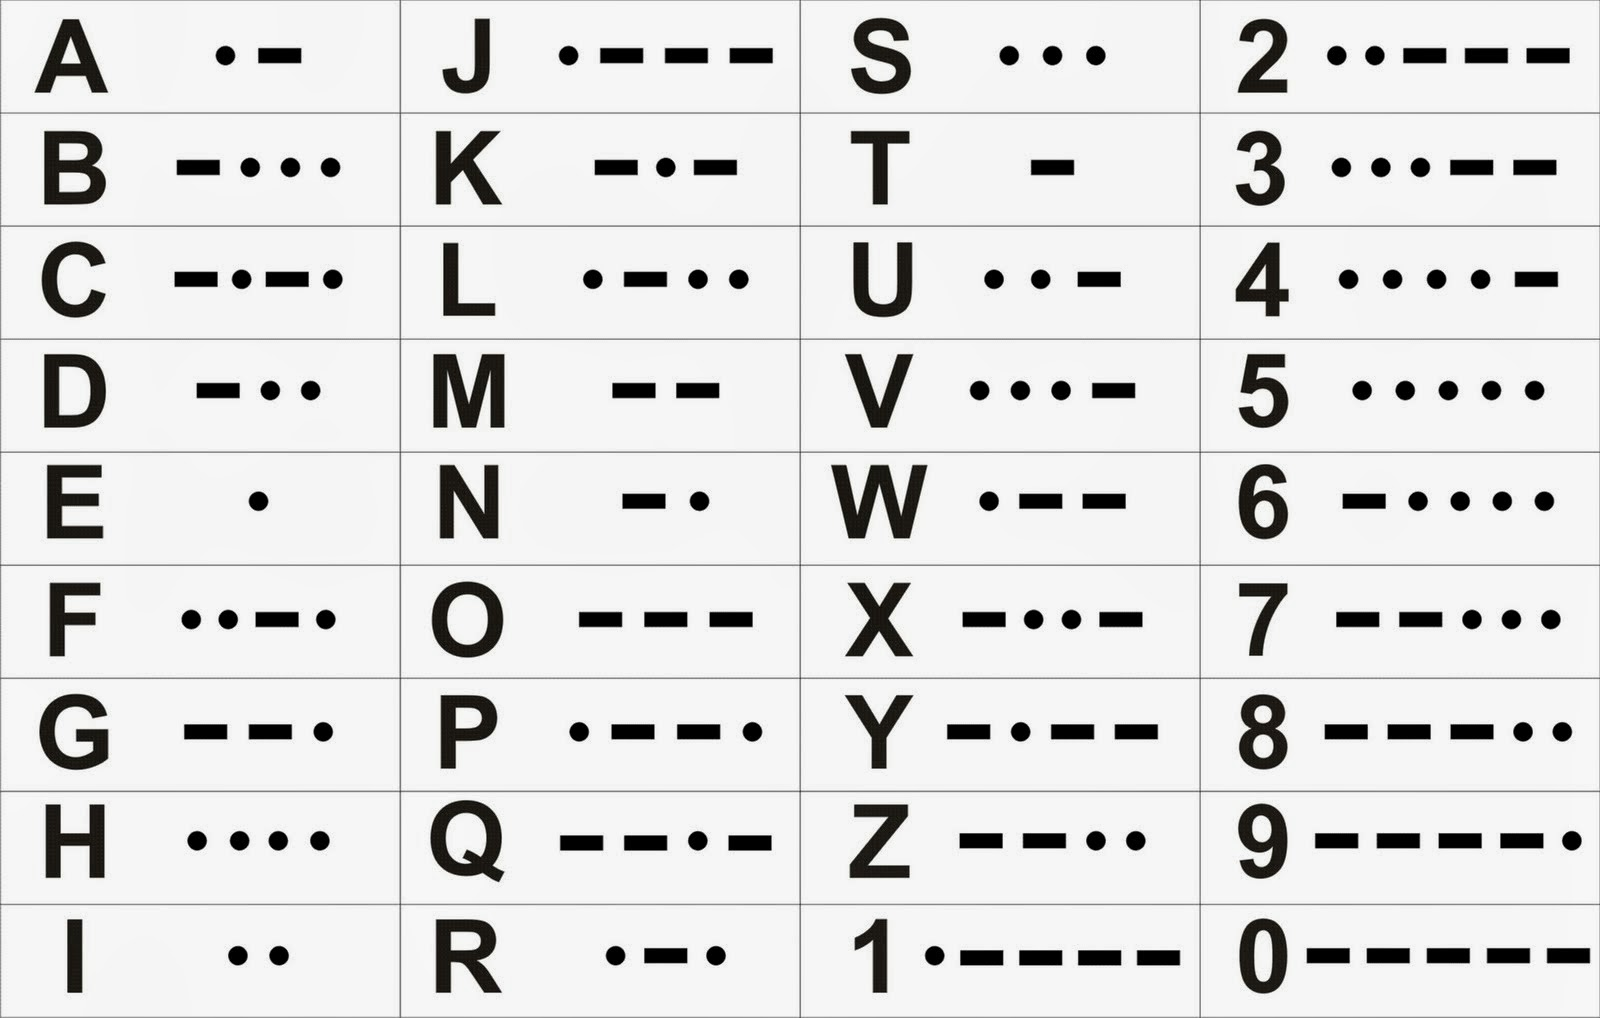
\includegraphics{assets/morse.jpg}
    \caption{morse}
\end{figure}

Possiamo trasformare una stringa in codice morse usando un dizionario
che associa ad ogni lettera la sua rappresentazione in codice morse. Per
creare la stringa in codice morse, iteriamo sulla stringa e per ogni
carattere prendiamo il suo valore nel dizionario. Attenzione, dobbiamo
prima convertire il carattere in maiuscolo, perché il dizionario
contiene solo le lettere maiuscole. Inoltre, dobbiamo usare la funzione
\texttt{get} per evitare che il programma restituisca un errore se la
lettera non è presente nel dizionario, in particolare come caso base
usiamo \texttt{""}.

\begin{tcolorbox}[breakable, size=fbox, boxrule=1pt, pad at break*=1mm,colback=cellbackground, colframe=cellborder]
    \prompt{In}{incolor}{59}{\boxspacing}
    \begin{Verbatim}[commandchars=\\\{\}]
        \PY{c+c1}{\PYZsh{} alfabeto morse}
        \PY{n}{morse\PYZus{}code} \PY{o}{=} \PY{p}{\PYZob{}}
        \PY{l+s+s1}{\PYZsq{}}\PY{l+s+s1}{A}\PY{l+s+s1}{\PYZsq{}}\PY{p}{:} \PY{l+s+s1}{\PYZsq{}}\PY{l+s+s1}{.\PYZhy{}}\PY{l+s+s1}{\PYZsq{}}\PY{p}{,} \PY{l+s+s1}{\PYZsq{}}\PY{l+s+s1}{B}\PY{l+s+s1}{\PYZsq{}}\PY{p}{:} \PY{l+s+s1}{\PYZsq{}}\PY{l+s+s1}{\PYZhy{}...}\PY{l+s+s1}{\PYZsq{}}\PY{p}{,} \PY{l+s+s1}{\PYZsq{}}\PY{l+s+s1}{C}\PY{l+s+s1}{\PYZsq{}}\PY{p}{:} \PY{l+s+s1}{\PYZsq{}}\PY{l+s+s1}{\PYZhy{}.\PYZhy{}.}\PY{l+s+s1}{\PYZsq{}}\PY{p}{,} \PY{l+s+s1}{\PYZsq{}}\PY{l+s+s1}{D}\PY{l+s+s1}{\PYZsq{}}\PY{p}{:} \PY{l+s+s1}{\PYZsq{}}\PY{l+s+s1}{\PYZhy{}..}\PY{l+s+s1}{\PYZsq{}}\PY{p}{,} \PY{l+s+s1}{\PYZsq{}}\PY{l+s+s1}{E}\PY{l+s+s1}{\PYZsq{}}\PY{p}{:} \PY{l+s+s1}{\PYZsq{}}\PY{l+s+s1}{.}\PY{l+s+s1}{\PYZsq{}}\PY{p}{,}
        \PY{l+s+s1}{\PYZsq{}}\PY{l+s+s1}{F}\PY{l+s+s1}{\PYZsq{}}\PY{p}{:} \PY{l+s+s1}{\PYZsq{}}\PY{l+s+s1}{..\PYZhy{}.}\PY{l+s+s1}{\PYZsq{}}\PY{p}{,} \PY{l+s+s1}{\PYZsq{}}\PY{l+s+s1}{G}\PY{l+s+s1}{\PYZsq{}}\PY{p}{:} \PY{l+s+s1}{\PYZsq{}}\PY{l+s+s1}{\PYZhy{}\PYZhy{}.}\PY{l+s+s1}{\PYZsq{}}\PY{p}{,} \PY{l+s+s1}{\PYZsq{}}\PY{l+s+s1}{H}\PY{l+s+s1}{\PYZsq{}}\PY{p}{:} \PY{l+s+s1}{\PYZsq{}}\PY{l+s+s1}{....}\PY{l+s+s1}{\PYZsq{}}\PY{p}{,} \PY{l+s+s1}{\PYZsq{}}\PY{l+s+s1}{I}\PY{l+s+s1}{\PYZsq{}}\PY{p}{:} \PY{l+s+s1}{\PYZsq{}}\PY{l+s+s1}{..}\PY{l+s+s1}{\PYZsq{}}\PY{p}{,} \PY{l+s+s1}{\PYZsq{}}\PY{l+s+s1}{J}\PY{l+s+s1}{\PYZsq{}}\PY{p}{:} \PY{l+s+s1}{\PYZsq{}}\PY{l+s+s1}{.\PYZhy{}\PYZhy{}\PYZhy{}}\PY{l+s+s1}{\PYZsq{}}\PY{p}{,}
        \PY{l+s+s1}{\PYZsq{}}\PY{l+s+s1}{K}\PY{l+s+s1}{\PYZsq{}}\PY{p}{:} \PY{l+s+s1}{\PYZsq{}}\PY{l+s+s1}{\PYZhy{}.\PYZhy{}}\PY{l+s+s1}{\PYZsq{}}\PY{p}{,} \PY{l+s+s1}{\PYZsq{}}\PY{l+s+s1}{L}\PY{l+s+s1}{\PYZsq{}}\PY{p}{:} \PY{l+s+s1}{\PYZsq{}}\PY{l+s+s1}{.\PYZhy{}..}\PY{l+s+s1}{\PYZsq{}}\PY{p}{,} \PY{l+s+s1}{\PYZsq{}}\PY{l+s+s1}{M}\PY{l+s+s1}{\PYZsq{}}\PY{p}{:} \PY{l+s+s1}{\PYZsq{}}\PY{l+s+s1}{\PYZhy{}\PYZhy{}}\PY{l+s+s1}{\PYZsq{}}\PY{p}{,} \PY{l+s+s1}{\PYZsq{}}\PY{l+s+s1}{N}\PY{l+s+s1}{\PYZsq{}}\PY{p}{:} \PY{l+s+s1}{\PYZsq{}}\PY{l+s+s1}{\PYZhy{}.}\PY{l+s+s1}{\PYZsq{}}\PY{p}{,} \PY{l+s+s1}{\PYZsq{}}\PY{l+s+s1}{O}\PY{l+s+s1}{\PYZsq{}}\PY{p}{:} \PY{l+s+s1}{\PYZsq{}}\PY{l+s+s1}{\PYZhy{}\PYZhy{}\PYZhy{}}\PY{l+s+s1}{\PYZsq{}}\PY{p}{,}
        \PY{l+s+s1}{\PYZsq{}}\PY{l+s+s1}{X}\PY{l+s+s1}{\PYZsq{}} \PY{p}{:} \PY{l+s+s1}{\PYZsq{}}\PY{l+s+s1}{\PYZhy{}..\PYZhy{}}\PY{l+s+s1}{\PYZsq{}}\PY{p}{,} \PY{l+s+s1}{\PYZsq{}}\PY{l+s+s1}{Y}\PY{l+s+s1}{\PYZsq{}} \PY{p}{:} \PY{l+s+s1}{\PYZsq{}}\PY{l+s+s1}{\PYZhy{}.\PYZhy{}\PYZhy{}}\PY{l+s+s1}{\PYZsq{}}\PY{p}{,} \PY{l+s+s1}{\PYZsq{}}\PY{l+s+s1}{Z}\PY{l+s+s1}{\PYZsq{}} \PY{p}{:} \PY{l+s+s1}{\PYZsq{}}\PY{l+s+s1}{\PYZhy{}\PYZhy{}..}\PY{l+s+s1}{\PYZsq{}}
        \PY{p}{\PYZcb{}}

        \PY{c+c1}{\PYZsh{} prendiamo una stringa}
        \PY{n}{s} \PY{o}{=} \PY{l+s+s1}{\PYZsq{}}\PY{l+s+s1}{Ciao come va? Tutto bene? Anche a te e parenti!}\PY{l+s+s1}{\PYZsq{}}

        \PY{c+c1}{\PYZsh{} creo la stringa in morse}
        \PY{n}{s} \PY{o}{=} \PY{p}{[}\PY{n}{morse\PYZus{}code}\PY{o}{.}\PY{n}{get}\PY{p}{(}\PY{n}{c}\PY{p}{,} \PY{l+s+s2}{\PYZdq{}}\PY{l+s+s2}{\PYZdq{}}\PY{p}{)} \PY{k}{for} \PY{n}{c} \PY{o+ow}{in} \PY{n}{s}\PY{o}{.}\PY{n}{upper}\PY{p}{(}\PY{p}{)}\PY{p}{]}

        \PY{c+c1}{\PYZsh{} unisco la lista in una stringa (in morse non ci sono spazi)}
        \PY{n}{s} \PY{o}{=} \PY{l+s+s1}{\PYZsq{}}\PY{l+s+s1}{\PYZsq{}}\PY{o}{.}\PY{n}{join}\PY{p}{(}\PY{n}{s}\PY{p}{)}

        \PY{n+nb}{print}\PY{p}{(}\PY{n}{s}\PY{p}{)}
    \end{Verbatim}
\end{tcolorbox}

\begin{Verbatim}[commandchars=\\\{\}]
    -.-{\ldots}-----.-.-----..-----{\ldots}-{\ldots}--.-.-{\ldots}-{\ldots}-.-{\ldots}
\end{Verbatim}

Usando questo stesso principio (e un po' di sintassi in più) possiamo
anche creare un programma che oltre a tradurre qualsiasi testo in codice
morse ne generi anche il suono.

Per esempio come questo sito qui:
\href{https://www.tetralark.com/MorsePy/}{MorsePy}

Che guarda un po' è stato scritto in Python! Link al
\href{https://github.com/Elucidation/MorsePy/blob/master/morse.py}{codice}.


% Add a bibliography block to the postdoc



\end{document}
